\documentclass[]{politex}
% ========== Opções ==========
% pnumromarab - Numeração de páginas usando algarismos romanos na parte pré-textual e arábicos na parte textual
% abnttoc - Forçar paginação no sumário conforme ABNT (inclui "p." na frente das páginas)
% normalnum - Numeração contínua de figuras e tabelas 
%	(caso contrário, a numeração é reiniciada a cada capítulo)
% draftprint - Ajusta as margens para impressão de rascunhos
%	(reduz a margem interna)
% twosideprint - Ajusta as margens para impressão frente e verso
% capsec - Forçar letras maiúsculas no título das seções
% espacosimples - Documento usando espaçamento simples
% espacoduplo - Documento usando espaçamento duplo
%	(o padrão é usar espaçamento 1.5)
% times - Tenta usar a fonte Times New Roman para o corpo do texto
% noindentfirst - Não indenta o primeiro parágrafo dos capítulos/seções


% ========== Packages ==========
\usepackage[utf8]{inputenc}
\usepackage{amsmath,amsthm,amsfonts,amssymb}
\usepackage{graphicx,cite,enumerate}
\usepackage{graphicx}
\usepackage{subcaption}


% ========== Language options ==========
%\usepackage[brazil]{babel}
\usepackage[english]{babel}


% ========== ABNT (requer ABNTeX 2) ==========
%	http://www.ctan.org/tex-archive/macros/latex/contrib/abntex2
%\usepackage[num]{abntex2cite}

% Forçar o abntex2 a usar [ ] nas referências ao invés de ( )
%\citebrackets{[}{]}


% ========== Lorem ipsum ==========
\usepackage{blindtext}



% ========== Opções do documento ==========
% Título
\titulo{EMG-driven Exoskeleton Control}

% Autor
\autor{Leonardo Fischi Sommer}

% Para múltiplos autores (TCC)
%\autor{Nome Sobrenome\\%
%		Nome Sobrenome\\%
%		Nome Sobrenome}

% Orientador / Coorientador
\orientador{Prof. Dr. Arturo Forner Cordero}
%\coorientador{Nome do coorientador (opcional)}

% Tipo de documento
%\tcc{Eletricista com ênfase em Sistemas Eletrônicos}
\dissertacao{Mechanical Engineering}
%\teseDOC{Engenharia Elétrica}
%\teseLD
%\memorialLD

% Departamento e área de concentração
\departamento{Mechanical Engineering}
\areaConcentracao{Control and Mechanical Automation Engineering}

% Local
\local{São Paulo}

% Ano
\data{2017}




\begin{document}
% ========== Capa e folhas de rosto ==========
\capa
\falsafolhaderosto
\folhaderosto


% ========== Folha de assinaturas (opcional) ==========
%\begin{folhadeaprovacao}
%	\assinatura{Prof.\ X}
%	\assinatura{Prof.\ Y}
%	\assinatura{Prof.\ Z}
%\end{folhadeaprovacao}


% ========== Ficha catalográfica ==========
% Fazer solicitação no site:
%	http://www.poli.usp.br/en/bibliotecas/servicos/catalogacao-na-publicacao.html


% ========== Dedicatória (opcional) ==========
\dedicatoria{Dedicatória}


% ========== Agradecimentos ==========
\begin{agradecimentos}

Thanks...



\end{agradecimentos}


% ========== Epígrafe (opcional) ==========
\epigrafe{%
	\emph{``Epígrafe''}
	\begin{flushright}
		-{}- Autor
	\end{flushright}
}


% ========== Resumo ==========
\begin{resumo}
Desenvolvimento de um método de controle para um exoesqueleto com um grau de liberdade, usando sinais de eletromiografia de superfície do usuário como sinal de entrada. A dinâmica tanto do exoesqueleto quanto do humano são estudadas para um melhor desenvolvimento do método de controle. Um exoesqueleto disponível é adaptado para servir de plataforma para os métodos de controle desenvolvidos. Três diferentes métodos de controle são avaliados e comparados nos quesitos de precisão e facilidade de uso. Os três métodos de controle desenvolvidos são: controle baseado em modelo matemático, controle proporcional e controle híbrido utilizando eletromiografia e sensores de força. Para o controle do motor do exoesqueleto também são desenvolvidos e comparados o controle de impedâncias e controle por modo de deslizamento.
%
\\[3\baselineskip]
%
\textbf{Palavras-Chave} -- Exoesqueleto, EMG, Controle proporcional, Identificação de sistemas.
\end{resumo}


% ========== Abstract ==========
\begin{abstract}
Development of a control system for an exoskeleton with one degree of freedom, using surface electromyography signals from the user as the input signal. Both the exoskeleton and the human dynamics are studied to better develop this control method. An available exoskeleton is adapted to serve as platform for the developed control methods. Three different control methods are evaluated and compared based on their precision and ease of use. The three developed control methods are: control based in mathematical model, proportional control and hybrid control using electromyography and force sensors. To control the exoskeleton motor two control methods were developed and compared: Impedance control and Sliding mode control.
%
\\[3\baselineskip]
%
\textbf{Keywords} -- Exoskeleton, EMG, Proportional control, System identification.
\end{abstract}


% ========== Listas (opcional) ==========
\listadefiguras
\listadetabelas

% ========== Sumário ==========
\sumario



% ========== Elementos textuais ==========

%\part{Introdução}
	
%\chapter{Capítulo com epígrafe}
%\capepigrafe[0.5\textwidth]{``Frase espirituosa de um autor famoso''}{Autor famoso}

%\blindtext

%\begin{citacaoLonga}
%	\blindtext
%\end{citacaoLonga}

%\blindtext



%\blinddocument

\part{Introduction}

\chapter{Introduction}
    
    \section{Objective}
    
    Design the control for one degree of freedom of an exoskeleton using sEMG signals from the user as the input signal. To accomplish this goal, three different control methods will be designed, evaluated and compared to determine which  one is more accurate and more easily controlled by the user. The three evaluated control methods will be: a model-based control, a proportional control and a hybrid control using sEMG and force sensors.
    
    An available exoskeleton will be adapted and the designed exoskeleton control will be applied.	    
    
    
    \section{Bibliographic Revision}
    
    In the United States, the number of people between the age of 18 and 64 that has some kind of movement disability has increased about 12\% between the years 1981 and 2014 \cite{VonSchrader2017}. Two of the main causes for disability are stroke and spinal cord injury. Yearly, 15 million people suffer stroke. From these, 5 million are fatal and 5 million cause a permanent disability. These number have been increasing in recent years and studies indicate these numbers will increase even further \cite{mackay2004atlas}. From 250 thousand to 500 thousand people suffer spinal cord injury yearly. The three main causes for spinal cord injury are traffic accidents, falls and violence. The non-traumatic injuries have been increasing in recent years. Moreover, with the rising in life expectancy of the world population \cite{UN}, the number of people affected by movement disabilities that difficult movement also raised.

	Due to these factors, the need for mechanisms that assist human movements have become more important. One of these mechanisms is the robotic exoskeleton.
    
	They are electromechanical structures coupled to physiological limbs, capable of doing or assisting movements. A robotic exoskeleton is usually composed of joints and rigid bodies \cite{pons2008wearable}.
There are several biological signals that can be used to control an external device. For exoskeleton control, that has the goal of moving a certain limb, it is interesting to use the same signals that are present in the human body, like the neural control signals responsible to activate the muscles. Since these signals cannot be accessed directly, the use of electromyography (EMG) has been explored to control these devices.
	
    The surface electromyography (sEMG) signal represents the electrical activity generated in muscle fibers in response to the activation provided by innervating motor neurons. The information present in the EMG signals is a composition of the synaptic inputs received by the motor neurons and the electrical properties from the muscle fibers \cite{Farina1215}.
    
     There are several other approaches to the control of a mechanical limb apart from the EMG signal. Among the relevant methods, some have been used in combination with EMG for the control of the prostheses or ortheses.
    

\subsection{EMG Control}

    Battye, Nightingale and Whillis \cite{Battye506} first proposed the use of proportional EMG control. The authors developed an apparatus capable of performing open and close actions according to when the test subject performed a grasp with his fingers. The apparatus consisted of: electrodes attached to the skin of the forearm; an electrical amplifier; a discriminator, which powered a solenoid when input signal was detected; the solenoid activated a hook, closing it. As a result, the authors were capable of designing a control system sensitive enough to close, and remain closed, when the test subject gripped a pencil in the fingers, regardless of the movement of other limbs. This concluded that the signal captured by the apparatus successfully eliminated the EMG signal from other muscles.
	
    Bottomley et al. \cite{Bottomley411} proposed another method for EMG-driven prostheses control. Two EMG electrode channels were placed on the forearm, one on the hand extensors and another on the hand flexors, to measure the muscle activity.  The signal from the muscles were amplified, rectified and smoothed. To remove the “cross-talk”, that is, the influence of the neighbor muscles on the targeted muscle, the signal of the neighbor muscle is subtracted from the signal obtained from the target muscle. These signals were used to control a Split hook capable of grasping objects, that exerted a force proportional to the EMG signal intensity. To control the desired force, a force sensor was attached to the hook. This device included a feedback control system that was capable of increasing, or decreasing, the Split hook grasping force compared to the measured EMG signal. When the force sensor detected zero force, that is, the hook is not grasping the object anymore and it is freely moving, the intensity of the EMG signal controlled the speed of the hook. A backlash generator was introduced in the electrical system, attenuating random variations when the signal changes exceeded a preset limit, that widens as the force feedback signal increases. The authors state that, after a few minutes wearing the apparatus, all the test subjects, even amputees, were able to control the hook in a graded manner.
    
    Similarly, Alter \cite{alter1966bioelectric} designed an exoskeleton control using two differential electrodes, one on the biceps and one on the triceps. Both signals were rectified and then the triceps signal was subtracted from the biceps signal. An adjustable lowpass filter was implemented. This signal was used as input signal to a power amplifier that powers an electric motor. Strain gauges were attached to the exoskeleton for force measurement, and the signal obtained from the strain gauges entered the system as a feedback signal. 
    
    Isidori and Nicolo \cite{Isidori1966} first described the myopulse processing technique, which was later developed by Childress et al. \cite{childress1971} and Philipson \cite{Philipson1985}. The myopulse processor works as follows: when the absolute value of the EMG surpasses a predetermined threshold value, the output of the processor turns on. This way, whenever the EMG activity rises, the duty cycle of the myoprocessor output will also increase. An illustration of this method can be seen in figure \ref{Myopulse Processor}.
    
    \begin{figure}[t]
      \centering
      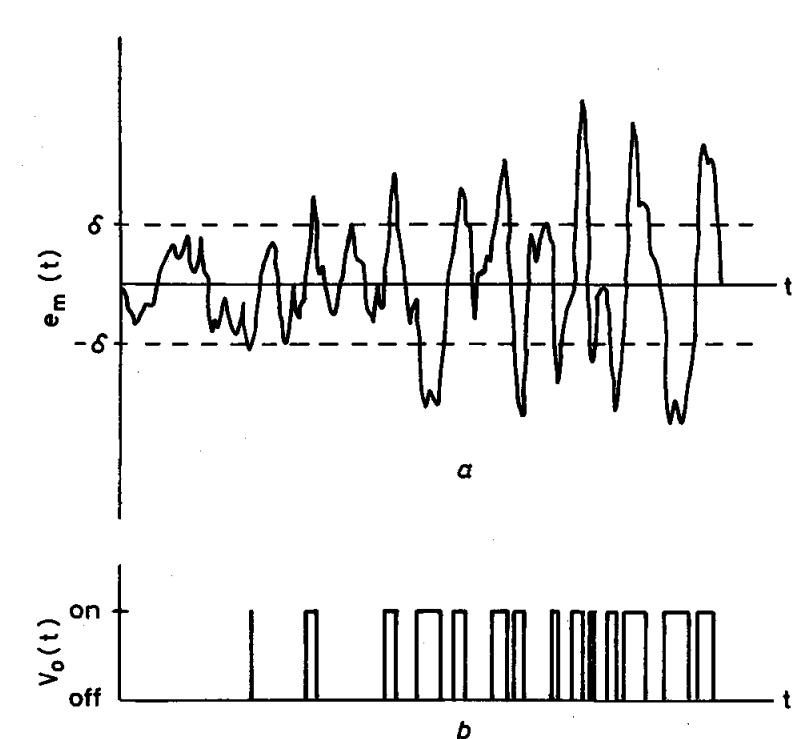
\includegraphics[scale=0.5]{Images/Myopulse.jpg}
      \caption{Illustration of the myopulse processing technique. The upper trace shows a typical bandpass-filtered EMG signal recorded with surface electrodes. The output will remain off as long as the absolute value of the EMG signal in the upper trace is below the level $\delta$, otherwise the output will be turned on. The lower trace illustrates the output from the myopulse processor \cite{Philipson1985}}
      \label{Myopulse Processor}
   \end{figure}
   
    In his system, two sets of electrodes were placed over the targeted muscle where the detection of electrical signal was desired. The EMG signal was sent to the myopulse processor, where the input signal was amplified and transformed into Pulse Width Modulated (PWM) signal. This PWM signal was sent to the microcomputer. Then, the microcomputer processed the PWM signals and sent the output signals to control the prosthetic arm according to the control algorithm. The myopulse processor is an electrical circuit composed of a dual comparator, with the value of the resistors defining the threshold value $\delta$.
    
    The signal measured through the EMG electrode is an analog signal, since it is a measure of the electrical activity of the muscle. To use this signal in a controller, it is needed to convert this signal to a digital signal.
    One advantage of this system is that, with the myopulse processor, there is no need for a conventional analog-to-digital converter. 
    The author also implemented a classification method for the prosthesis control. Different from the previous control methods, where the actuation of the joint was proportional to the intensity of EMG signal, this system can perform different movements. In this work, by measuring the intensity of EMG signals from two electrode sets, the author was capable of achieving seven different movements. Figure \ref{Movement space} shows the proposed dynamic area for the prostheses control. According to the intensity of the input from the two target muscles one of the seven possible actions is performed.
    This control system was applied to a prostheses and tested on four amputees subjects. With proper training sessions, the amputees were able to perform some daily tasks such as grasping a plastic cup containing water, pour the desired amount and then release the cup. In the case of the nonamputees, the subjects could achieve good control over the seven-state control system. 
    
    \begin{figure}[thpb]
      \centering
      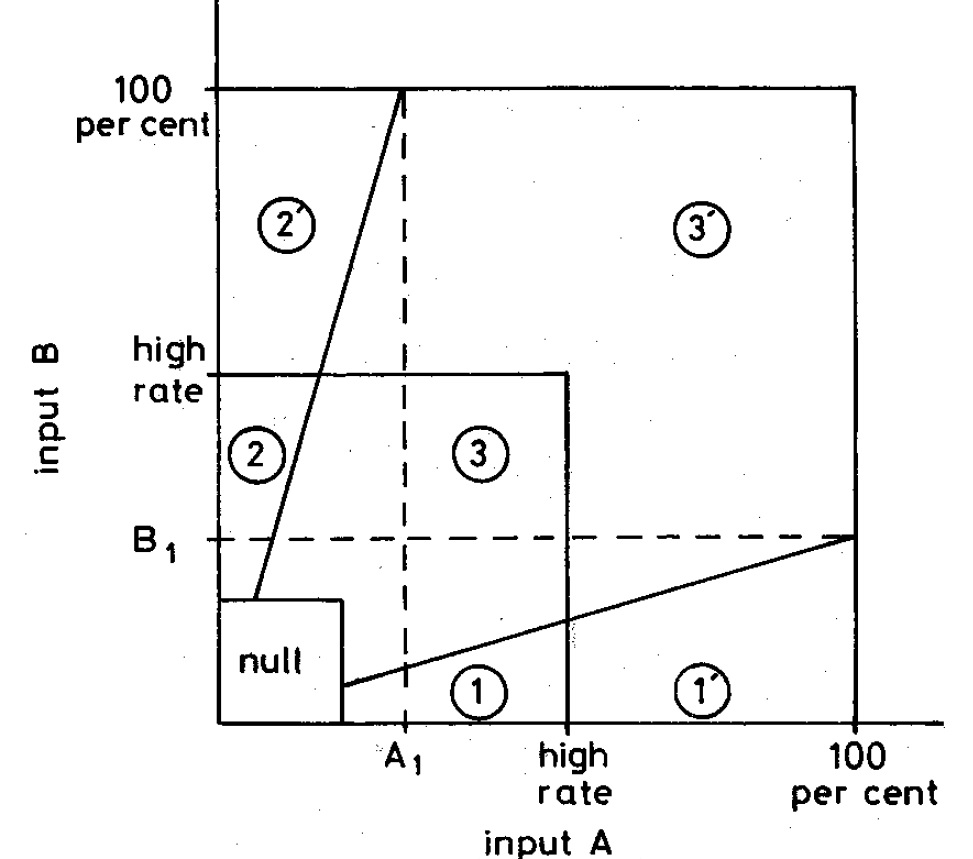
\includegraphics[scale=0.5]{Images/Movement_Area_-_Philipson.jpg}
      \caption{Diagram showing the possible movement areas according to the muscle inputs \cite{Philipson1985}}
      \label{Movement space}
   \end{figure}
   
   Parker et al. \cite{Parker1977662} sought to develop a better processor for the EMG signal, that is, find the signal processor that achieves the minimum error at selecting the desired action for the prostheses. The authors developed a model that extracts the relevant information from the myoelectric signal obtained by a bipolar electrode configuration. One of the main points of this model is that the pooled motor unit firing rate reflects the contraction level and is thus the information parameter in the myoelectric signal. Hogan \cite{4123279,4123280}, also in search of a better myoprocessor, developed a similar mathematical model to estimate muscle force based on EMG signal. 
    
    The myoelectric signal is a zero-mean stochastic process. To estimate the user's control signal, it is necessary to add a nonlinearity to the estimator. Typically, a full-wave rectifier is used for this nonlinearity, followed by a low pass filter. Evans et al. \cite{4121805} proposed another model based approach to this EMG control problem. The authors used a logarithmic nonlinearity, followed by a a linear minimun mean-square error in the EMG-force estimation. This way it was possible to add a Kalman filter to estimate the control signal. 
    
     Hudgins \cite{Hudgins204774} proposed a control strategy for a multifunction prosthesis based on the classification of myoelectric patterns into different movements. Initially, the author conducted tests on both healthy subjects and amputees. The test consisted of an isometric contraction with constant force and a contraction (e.g. flexion, extension, etc.) with no constraints related to force, velocity or range. The subjects were asked only to make consistent motions, starting from a comfortable neutral position.
     
     By taking the average of the EMG signal for the first 300ms to 600ms of the movement, that is, the onset of the movement, it was possible to detect different signal patterns for each movement (e.g. elbow flexion, elbow extension, forearm supination, etc.) shown in figure \ref{EMG patterns}. Other control schemes, based on steady state levels, are limited to only three limb functions: for an elbow mechanism, one can only control extension, flexion and the off-state. The scheme proposed by Hudgins targets the EMG signal of only one muscle and is capable of assigning as many functions as the number of distinct signal patterns generated by the muscle.
     
         \begin{figure}[thpb]
      \centering
      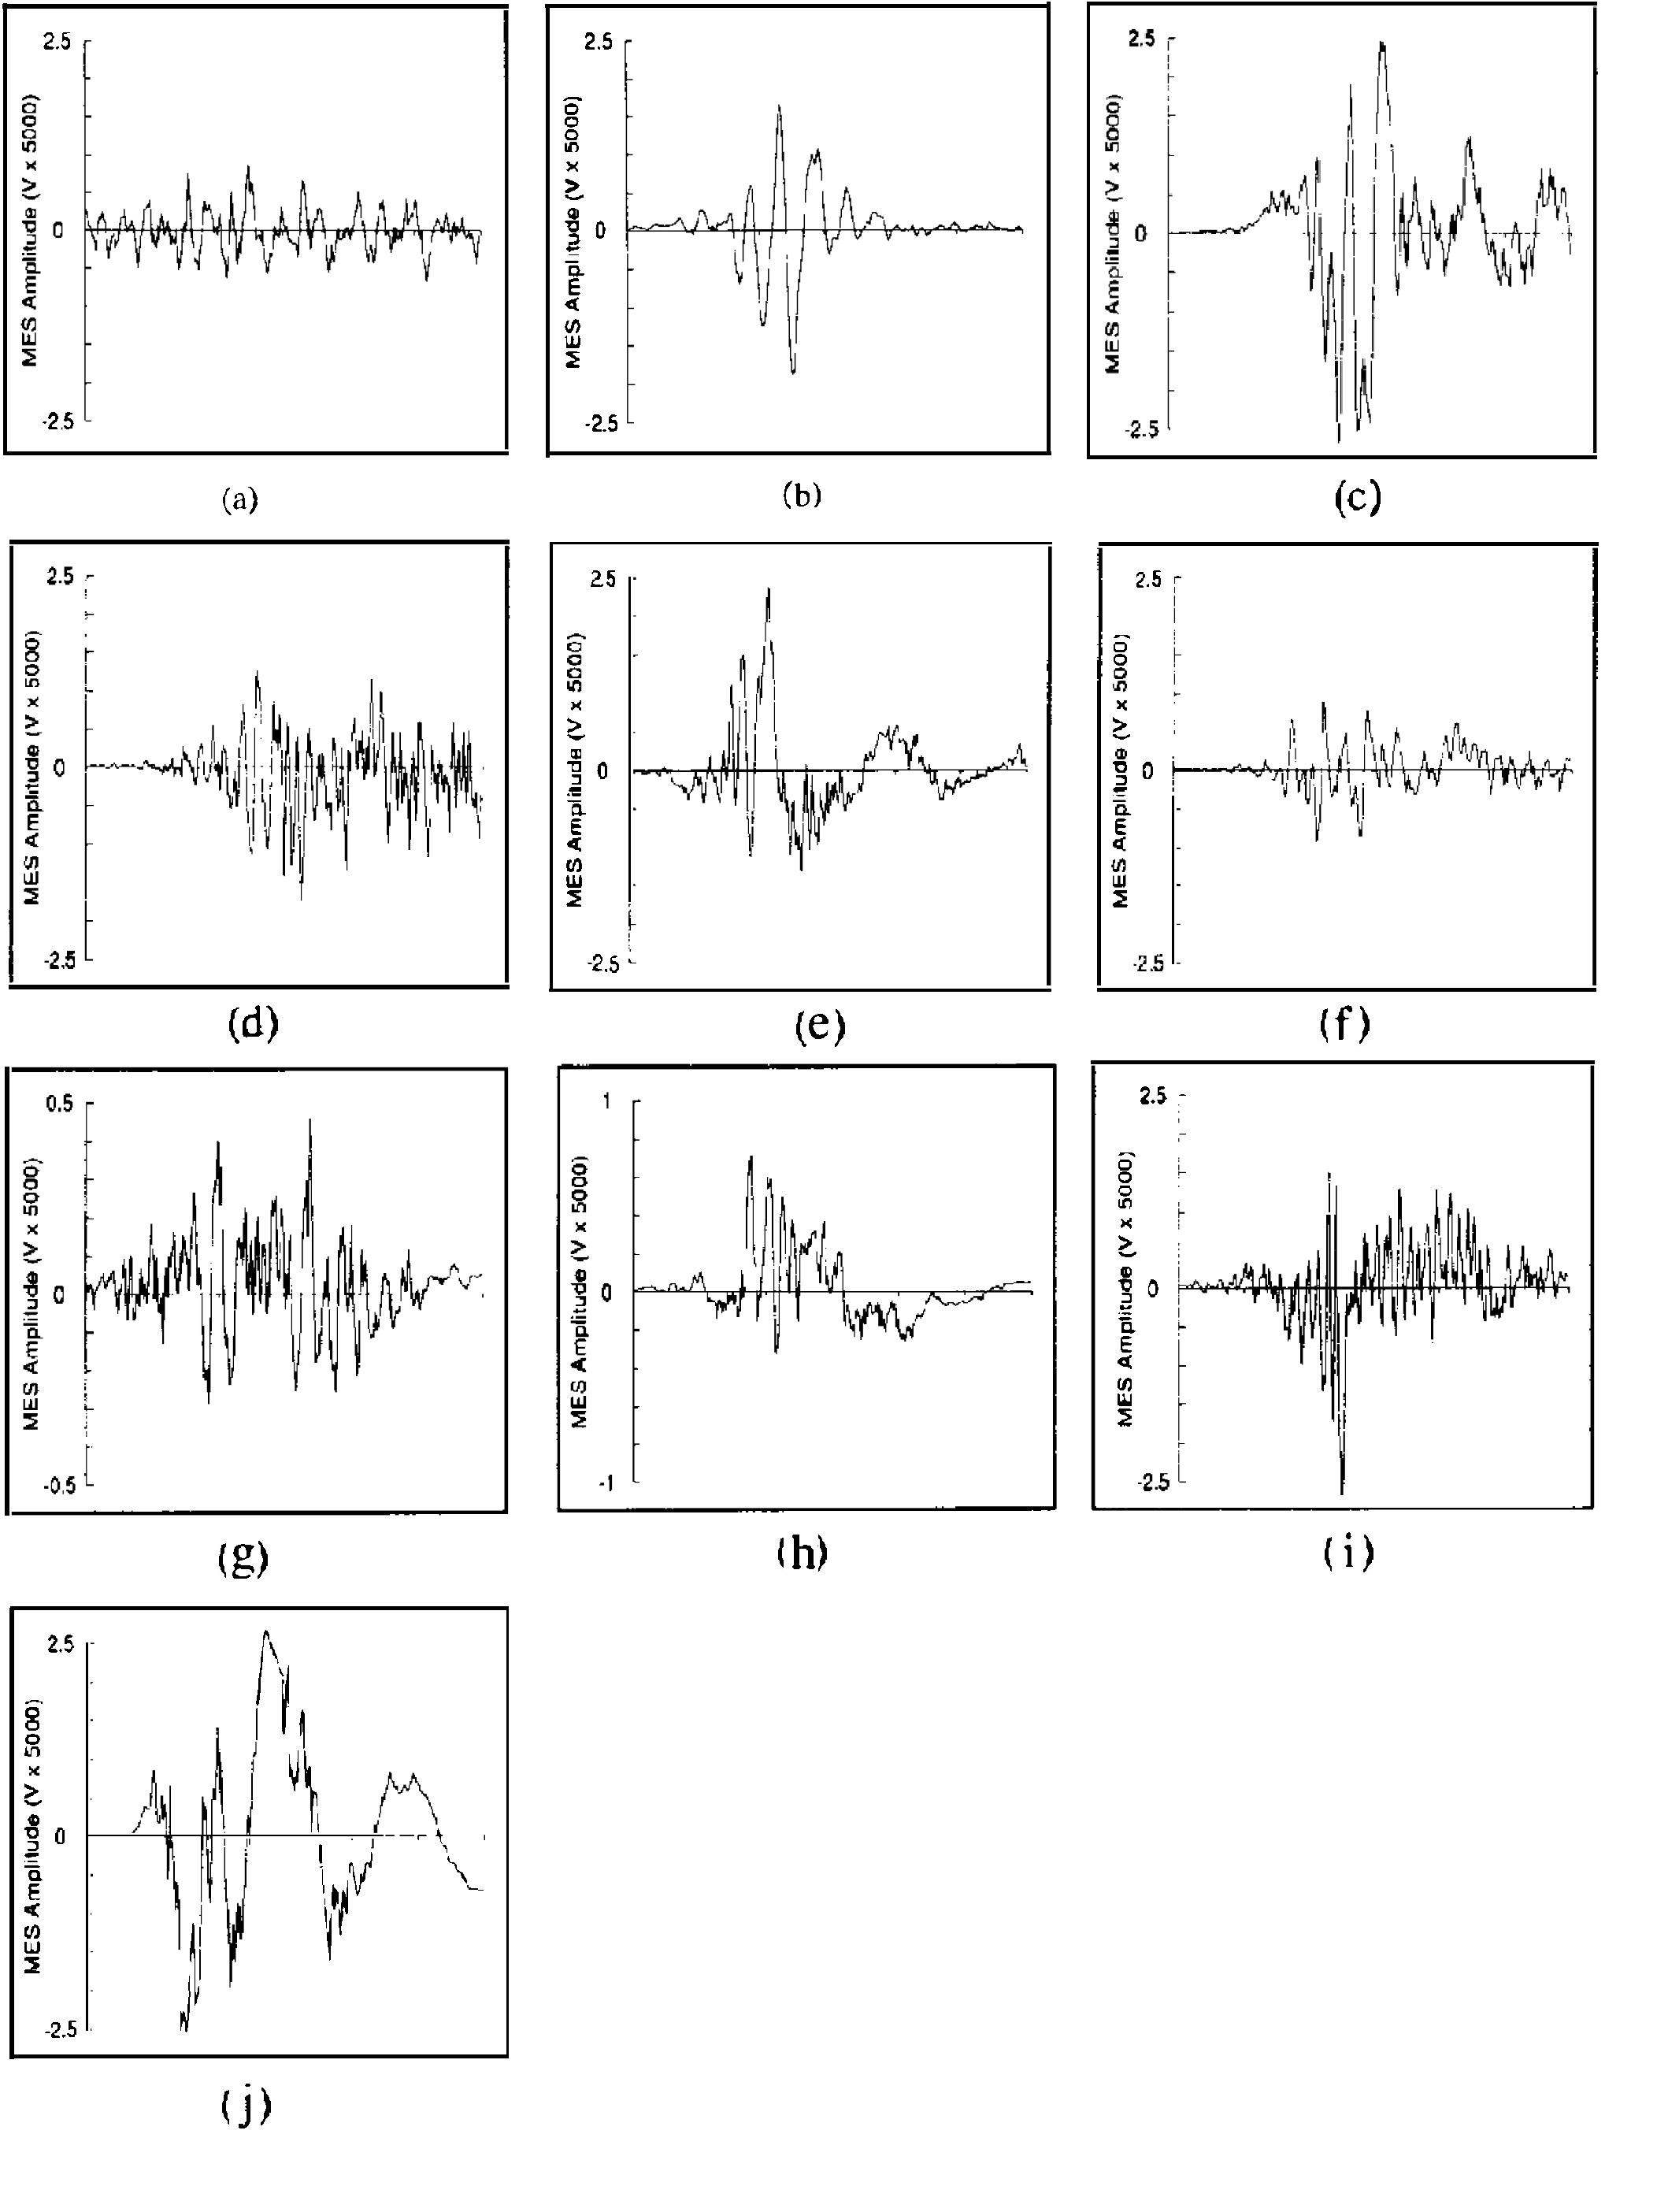
\includegraphics[width = \textwidth]{Images/EMG_patterns.jpg}
      \caption{Average of the first 300ms of the EMG recordings for the following movements: For a normally limbed subject: a) Isometric contraction; b) elbow flexion; c) Forearm supination; d) elbow extension; e) wrist flexion; f) forearm pronation; for the amputee subject: g) inward humeral rotation; h) contraction of the flexor muscle group; i) contraction of the extensor muscle group and j) biceps/triceps co-contraction. Adapted from \cite{Hudgins204774}}
      \label{EMG patterns}
   \end{figure}
   
   Since the prosthesis is capable of performing different movements, it is necessary to implement a classifier, that is, a method that chooses the desired movement or action based on the input signal. An Artificial Neural Network (ANN) was chosen as the classifier. The authors proposed a group of parameters, called features, which served as input to the classifier. The following features were chosen to represent the myoelectric patterns: Mean Absolute Value (MAV): it is the mean value of the signal throughout the data segment; Mean Absolute Value Slope: is the difference between the MAV of each segment; Zero Crossing (ZC): number of times the waveform crosses the zero value (it is needed to add a "dead-zone" to the signal to avoid noise inducted zero crossings); Slope Sign Changes (SSN): the number of times the slope of the waveform changes sign (the same "dead-zone" applied previously must be applied here); Waveform Length (WL): is the cumulative length of the waveform throughout the data segment. By using these previous features, one can get values for waveform amplitude, frequency and duration within a single parameter. This classification method has become known as the Time Domain feature set \cite{Johnny2009}.
   
   Tests showed that the subjects were capable of performing up to four different movements with an accuracy ranging from 70-95\%, before training. However, a major drawback from this control scheme is that, since the classification method only considers the movement onset, the EMG signal must always start from a resting position. If the user tries to switch from one movement to another in a period of time smaller then the averaging window (300ms-600ms), the control scheme will fail.
   
   Englehart \cite{Englehart1999431}, further developing the pattern recognition problem, tested some time-frequency-domain sets  for the EMG signal processing. The sets used were: Short-time Fourier Transform (STFT), Wavelet Transform (WT) and Wavelet Packet transform (WPT).
   
   The same group also proposed a method  to overcome the previous problem regarding the fast transition between two different movements \cite{Englehart1206493}. To do so, instead of segmenting the EMG data into multiple frames for classification, now the data was acquired continuously on a single, unsegmented window. In this scenario, the data acquired from 12 subjects were compared using the Time Domain statistics and using the time-frequency-domain sets. The Time Domain sets outperformed the time-frequency-domain sets in continuous data acquisition.
   
   Jiang \cite{Jiang4663628} proposed a method to estimate force from the Mean Square Value (MSV) of the EMG signal. MSV is defined as the mean value of the square of the signal throughout the data segment. By stating that it is possible to maintain the muscle cross-talk at low levels, it is possible to determine a direct relationship between muscle force and sEMG measurements.
   
   \subsection{Hybrid Control and Other Control Modalities}
   
   \subsubsection{Hybrid Control}
     
   If the subject had some residual shoulder movement it is possible to combine a joystick at the shoulder with EMG for a movement classification method \cite{Losier4353750}. The system was capable of performing nine different activities. Eight of then were controlled by the position of the shoulder and one by EMG input when the user performed a humeral rotation movement. The Time Domain technique was used to differentiate the EMG readings from humeral rotation from the normal shoulder movements.
   
   Fougner and Stadvahl \cite{Fougner2008}\cite{Fougner2011} used force sensors on the EMG electrodes to measure external forces. This application is useful for the cancellation of artifacts caused by these forces (e.g. movement artifacts). 
   
   Fougner \cite{Fougner5985538} noted that different limb positions associated with daily activities can affect the EMG signal results. To overcome this problem, the EMG signal was associated with accelerometers placed at the user's forearm and biceps. This allows the pattern recognition system to know the position and orientation of the limb, compensating for eventual changes on the EMG signal.
   
   \subsubsection{Other Control Modalities}
   
   If EMG sensors are difficult to place or cause discomfort to the user it is possible to use other techniques like Mechanomyography (MMG). Silva \cite{Silva1280527} used MMG for a classification method control strategy. Mechanomyography is the measurement of the mechanical vibrations caused by the contraction of the muscle. In this case, the MMG sensors were used as a substitute of the EMG sensors, when the EMG sensors are of difficult placement or unconfortable for the patient. This method can also be referred as phonomyogram, vibromyogram, soundmyogram or acoustomyogram, since the sensor is composed of a microphone and an accelerometer that detect the air vibration between the sensor and the target muscle. 
   
   Kenney \cite{Kenney1999589} used the dimensional change of the muscle as control signal for his control strategy. This technique is called Myokinemetric. The author designed a sensor, composed by a Hall Effect sensor and a permanent magnet. The relative distance between these two components varied according to the dimensional change of the subject's muscle. To validate this strategy a tracking test was performed, where the test subject was supposed to track a signal presented on a screen by controlling the dimension of his muscle.
   
   Stadvahl \cite{Standvahl1997} used ultrasound to create a force estimation. As the muscle contracts, the shape of the muscle changes. The ultrasound, when transmitted to a medium, generates an echo signal that can be acquired through an ultrasound sensor. Using this information, it is possible to determine a relation between the ultrasound and the force through the Cross Correlation technique. Chen \cite{Chen2011} attached ultrasound transducers to the subject's forearm to estimate the wrist angle using the ultrasound signal. 
   
   Nightingale \cite{NIGHTINGALE1985167} used force and slip sensors on the Southampton Hand to detect forces applied to the hand and relative slipping motion between the hand and objects. By using the force and slip sensors paired with an EMG control, state machine control logic could be implemented. According to the EMG signal magnitude the control logic would open or close the hand and through the force sensors measurement it was possible to asses more specific states for the hand movement, like holding or squeezing an object.
   
   \subsection{State-of-the-Art of Exoskeletons and Exoskeleton Control}
   
   The exoskeletons can be divided according to their applications: performance enhancement, haptic interfaces, remote operation, functional assistance (active orthoses and prostheses), rehabilitation and motor control exploration. In this work two groups will be focused: the performance enhancement and the functional assistance. The performance enhancement exoskeleton allows healthy users to perform a difficult task by either reducing the forces or the expended energy, or perform a task that is impossible to accomplish by human strength or skill, solely. The functional assistance assists the user by modifying or recovering the motor function of the neuromuscular and skeletal system. However, this distinction, in some cases, can be not as clear \cite{Dollar4456745}.
   
   One of the major incentives to the development of exoskeleton has been the Exoskeletons for Human Performance Augmentation (EHPA), a program supported by the Defense Advanced Project Agency (DARPA). This program is developing exoskeletons capable of increasing the capabilities of ground soldiers beyond that of a human. There are three critical technologies that are the focus of this program: Energy, power and actuation; controls and haptic interface; design and integration \cite{Ephraim2002822}.
   
   HAL (Hybrid Assistive Limb) is an exoskeleton focused on both performance-augmenting as well as rehabilitation \cite{Sankai2011}. The HAL-5 is a full-body exoskeleton. The joints are powered by DC motors with harmonic drives placed directly on the joints. Attached to the exoskeleton is an special shoe with ground reaction force sensors. It is attached to the user by harnesses at the hip, thighs, calves, upper arms and forearms, as well as the shoe. 
   
   The HAL-5 utilizes a broad range of sensors for its controlling. The intention detection is done primarily by sEMG sensors. As soon as the EMG level exceeds a threshold, the motion support is triggered. An assistive torque is provided to the user. This torque is composed of three parts: an assistive torque; a viscous torque that prevents high velocity motions, maintaining safety; and a gravity compensating torque \cite{kawamoto2010}. In some experiments, the motion intention detection was done by the ground reaction sensor, to adapt the exoskeleton for patients with spinal cord injury. When the user shifts its weight to the next stance leg, the reaction force on this leg is higher that the other, triggering the exoskeleton motion \cite{Tsukahara2015}. Also, there are potentiometers, gyroscopes and accelerometers for the measurement of the angle, speed and acceleration of limbs and joints.
   
   \begin{figure}[thpb]
      \centering
      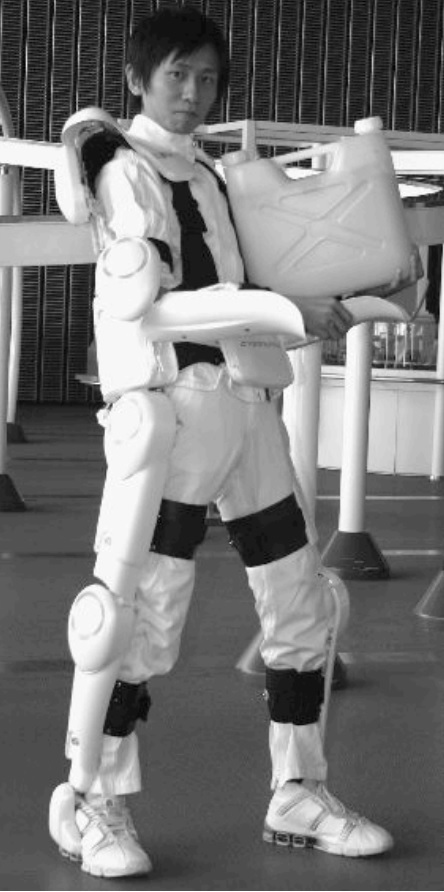
\includegraphics[scale=0.4]{Images/HAL5.jpg}
      \caption{HAL-5 exoskeleton \cite{Sankai2011}}
      \label{HAL5}
   \end{figure}
   
   In \cite{Otsuka6181399} the authors further developed the HAL upper-limb exoskeleton for meal assistance. It is composed of a shoulder joint with three degrees of freedom and an elbow joint with one degree of freedom. Also, a grasp assistance mechanism is attached to the forearm to allow for manipulation of objects by the user.
   
   One interesting aspect of the HAL exoskeleton is its modularity. Currently, there are separated products for upper-limbs, lower-limbs, lumbar support, as well as other modalities, like a heavy-duty and a disaster recovery exoskeleton \cite{cyberdyne}.
   
   The manufacturer states that the full-body HAL-5 weighs approximately 23kg, has a continuous operating time of approximately 2 hours and 40 minutes and is capable of lifting objects up to 70kg. The HAL\textsuperscript{\textregistered} exoskeleton is capable of performing different activities such as standing up from a chair, walking and climbing up and down stairs.
   
   The HAL\textsuperscript{\textregistered} exoskeleton is already used in many medical institutions in Japan and already received certification for clinical use in Europe. It is commercialized by Cyberdyne Inc.   
   
   
   
   The Berkeley Lower Extremity Exoskeleton (BLEEX), funded by the DARPA, is a self-powered exoskeleton that enhances the strength and endurance of a human \cite{Kazerooni2006}. 
   
   \begin{figure}[thpb]
      \centering
      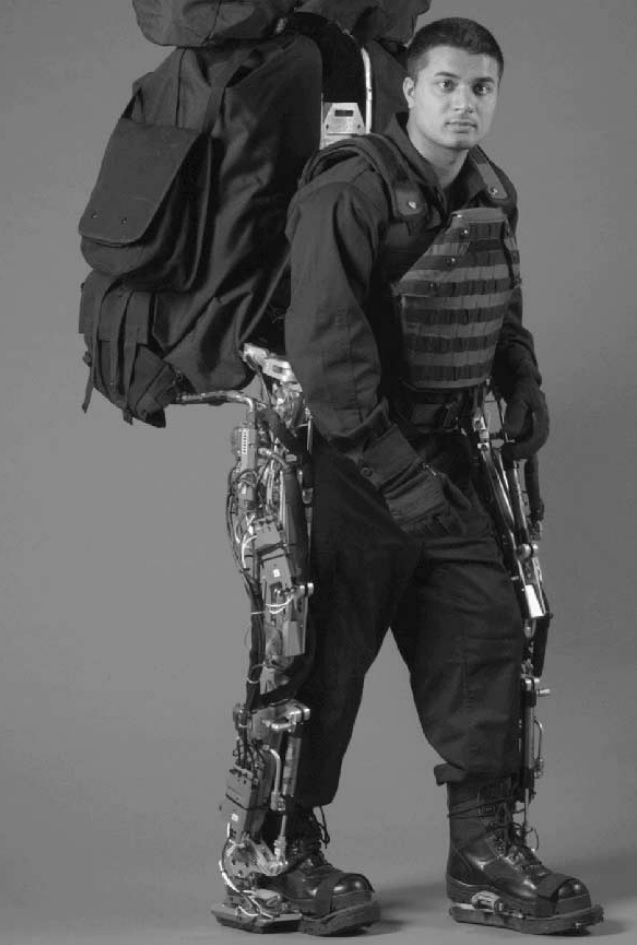
\includegraphics[scale=0.4]{Images/BLEEX.jpg}
      \caption{University of California at Berkeley's BLEEX exoskeleton \cite{Zoss1618670}}
      \label{BLEEX}
   \end{figure}
   
   The BLEEX exoskeleton has 7 degrees of freedom (DOF) per leg: 3 DOF at the hip, 1 DOF at the knee and 3 DOF at the ankle. For the hip, both the flexion/extension and the abduction/adduction joints are aligned to the human joint, but the rotation joint is positioned behind the user and under the torso. The reason is that, an aligned rotation joint would result in limited ranges of motion and singularities in some of the human postures. For the ankle, the flexion/extension axis coincides with the human ankle joint, but the abduction/adduction and rotation axis do not coincide with the human joint axis and form a plane outside of the human's foot. The front of the foot is compliant, allowing the flexing of the user's toes. The exoskeleton is only rigidly connected to the user at the hip and the foot \cite{Zoss1618670}.
   
   The BLEEX structure and actuation was designed based on the clinical gait analysis (CGA) of an 75-kg person. Analyzing the CGA, it was possible to determine which exoskeleton joint required actuation, based on the joint torque and power during gait. From this analysis, it was determined that the flexion/extension joints of hip, knee and ankle and the abduction/adduction joint should be actuated. 
   
   Initially, the selected actuator for the BLEEX was double-acting linear hydraulic actuators. They are compact in size, low weight and capable of exerting high forces. The actuators are placed in a triangular disposition in relation to the joint, resulting in a torque that varies according to the joint angle \cite{Chu1570789}.
   
   The average power consumption of the BLEEX during the walking cycle is 1143 W, compared to 165 W of mechanical power exerted by the human during normal gait. This exoskeleton is capable of supporting up to 75 kg and walk at speeds up to 1.3 m/s.
   
   In a later study, it was analyzed the feasibility of using electrical motors instead of the previous hydraulic ones. The designed electrical motors weighed an average of 4.1 kg opposed to the 2.1 kg hydraulic actuators. While the electric actuator weight is all centered in the actual joint, about 40\% of the weight hydraulic actuator is located away from the joint. At test performed at ground-level walking at the speed of 1.3 m/s, it was measured that the actuator power consumption was 598 W. Comparing both actuators, the electrical actuator is 95\% heavier and 92\% more power efficient \cite{Zoss2006}.
   
   An hybrid Hydraulic-Electric Power unit (HEPU) was designed in the attempt to provide autonomous energy for the exoskeleton. The hydraulic energy would supply the necessary mechanical parts of the exoskeleton, while the electrical energy would power the computer, sensors and other peripherals. Even though the designed HEPU could provide the necessary requirements of electrical and hydraulic power, it exceeded in both weight and noise output. The desired weight and noise output were 23 kg and 78 dBA, respectively. The achieved values were 30 kg and 87 dBA \cite{Amundson2006DevelopmentOH}.
   
   The control of the BLEEX exoskeleton has no sensors attached to the user. Every sensor is located only on the exoskeleton. It uses the forces applied by the environment and the user to the exoskeleton as the control signal \cite{Steger1642232}. The inverse dynamics of the exoskeleton are used as a feedback so that, when accounting the user force, the control loop gain approaches an unitary value. This control strategy has two main advantages: it allows for wide bandwidth maneuvers, necessary since the exoskeleton needs to respond to a wide variety of the human's movements; it is independent to changes in the user dynamics. The tradeoff of this control strategy is that it needs an accurate model of the exoskeleton dynamics. To address this, experiments in \cite{Ghan1642233} applied system identification methods to calculate the exoskeleton dynamics.
   
   One of the most well-established exoskeletons for disabled users is the ReWalk\textsuperscript{TM}. The ReWalk\textsuperscript{TM} is a lower extremity, battery powered exoskeleton that allows individuals with thoracic or lower level motor complete spinal cord injury to walk independently. It is suitable for adults who have preserved bilateral upper extremity function. The user must be using crutches to maintain balance. The mechanical structure is composed of bilateral supports parallel to the thighs and legs, articulated at the knee and hip. A rigid shoe insert fixes the user's feet. Velcro closures distributed at the legs and thighs and a waist belt secure the attachment between user and exoskeleton. The computer-based controller and the batteries are stored within a backpack. A tilt sensor is placed at the exoskeleton structure, near the waist \cite{Esquenazi2013}.
   
   The active joints of the ReWalk\textsuperscript{TM} are the knee and waist joint. The ankle joint is passive joint with spring-assisted dorsiflexion. The exoskeleton has five different operation modes. walk, sit-stand, stand-sit, up steps and down steps. In the 'walk' mode, the stepping procedure is triggered by the forward flexion of the upper body, measured by the tilt sensor. The maximum walking velocity is 2.2 km/h. The mode selection can be made through an user-operated wrist pad. There is also the option to manually control the position of the lower limbs \cite{Zeilig2012}. 
   
   \begin{figure}[thpb]
      \centering
      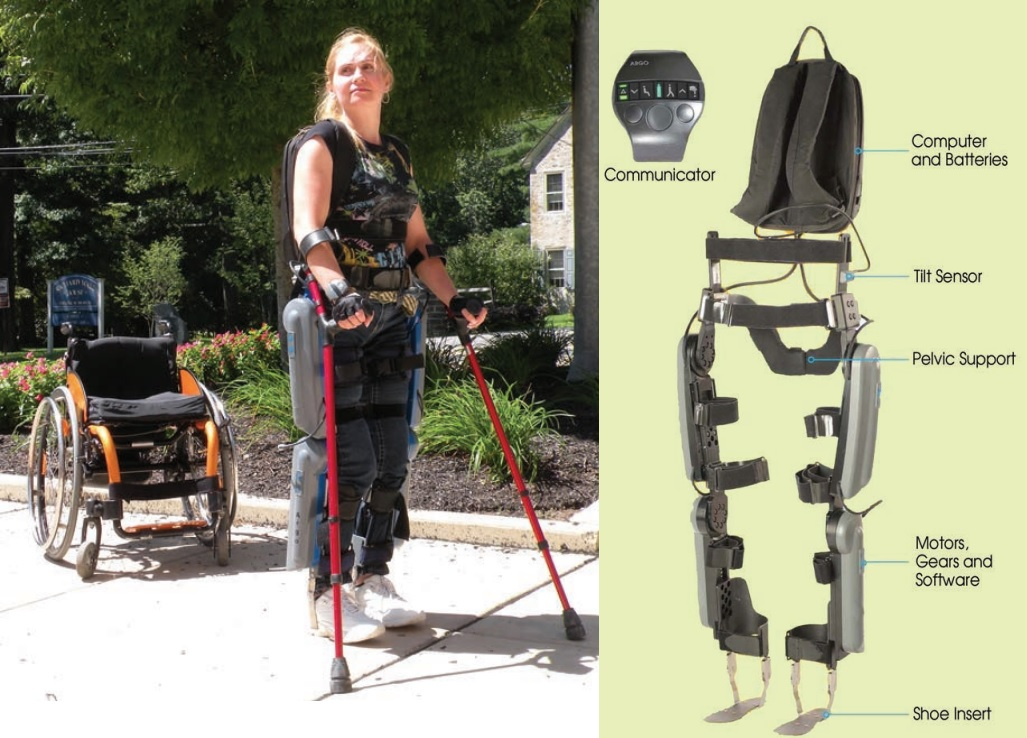
\includegraphics[scale=0.5]{Images/ReWalk.jpg}
      \caption{The ReWalk\textsuperscript{TM} exoskeleton worn by an user and its basic structure \cite{Esquenazi2013}}
      \label{ReWalk}
   \end{figure}
   
   Some studies have been performed with the ReWalk\textsuperscript{TM} \cite{Zeilig2012} \cite{Fineberg2013} \cite{Talaty6650469}. Overall the participants of the test were satisfied with the device, being able to walk without falling. The volunteers reached the level of being able to walk 100m with the use of crutches. However, they have not attained proficiency to use the device on a daily basis. It is stated that the users found relative difficulty with wearing and adjusting the device.   
   
   Even tough many advancements in this area have been made, the effective use of an exoskeleton continues to be extremely difficult. Even though many technologies have been advertised lately, there is a lack of quantitative studies available to researchers \cite{Young7393837}.
   
   The MIT exoskeleton, a quasi passive exoskeleton concept, explores the passive dynamics of human walking trying to achieve a lighter and more efficient exoskeleton. Although, tests performed show that the total metabolic cost of walking increased when used the exoskeleton while carrying a load, compared to no exoskeleton being used while carrying the load in a backpack. The increase in metabolic cost was found to be 10\% higher  \cite{Walsh2007}. Although, test participants stated that carrying the load while wearing the exoskeleton was more comfortable compared to carrying the backpack alone \cite{Valiente2005}. Another study demonstrated the exoskeleton is capable of transferring up to 90\% of the load to the ground, depending on the gait phase, but increases the metabolic cost in a range from 32\% up to 74\%, depending on some variations of the mechanical structure and actuation of the exoskeleton \cite{Walsh2006}.
   
   It has been previously studied that one of the major problems of ambulation devices for paraplegics is the high-energy demands imposed to the user. Franceschini et al. \cite{FRANCESCHINI1997582} conducted a survey on patients that utilized reciprocating orthoses (ARGO, RGO, HGO). From the 74 patients, 24 patients abandoned the use of the mechanism by the end of the study. One of the main reasons was the excessive energy cost.

\mypart{Exoskeleton Platforms}{In this part, it is described the work developed on the mechanical design of the exoskeleton platforms that will be used to implement the control strategies developed}

\chapter{Trunk and Lower Limb Exoskeleton for Stable Autonomous Walking (ETMICAE)}

\section{Description}

The ETMICAE is a bipedal trunk and lower limb exoskeleton to assist the walking movement of people with motor disabilities. It allows the use of the exoskeleton for people that cannot mantain a full control of the body and lower limbs. It includes human gait stability control.

It is currently being developed at the Biomechatronics Laboratory - Mechanical Engineering and Mechanical Systems Department - Politechnic School of the University of São Paulo (USP). This project is being developed in collaboration with the Rehabilitation Medicine Institute of the Clinics Hospital - Medicine School of USP, São Carlos School of Engineering (EESC-USP).

When the project is completed it will mainly contribute in two major areas: Clinical studies and technological studies. For clinical studies, the ETMICAE will be transfered to a clinic to test and evaluate the exoskeleton on test subjects with motor disabilities. For the technological studies, the exoskeleton will act as platform for testing of mechanical, electrical and control technologies developed at the Biomechatronics laboratory. 

\section{Mechanical Structure}

The author of this thesis was responsible in designing the hip, thigh, knee and leg mechanical structure, as well as its coupling components. The explanation of this design is described in this section.

\subsection{Hip}

\subsubsection{Description}

The hip of the exoskeleton will have four degrees of freedom, being the abduction/adduction and flexion/extension of both thighs. The exoskeleton will not have the pronation/supination movement of the thighs.

The hips are composed of the following parts:

A base will will attach the hip of the exoskeleton to the support of the motors, located at the back of the user.

\begin{figure}[thpb]
      \centering
      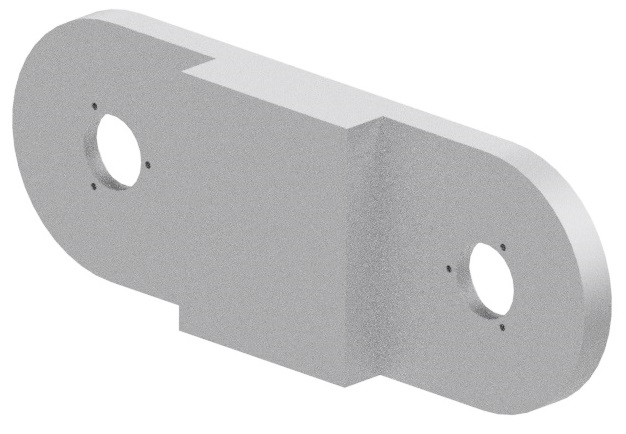
\includegraphics[width=0.4\textwidth]{Images/Base.jpg}
      \caption{Base}
      \label{Base}
   \end{figure}
   
Attached to the base there are two joints that will perform the abduction/adduction degree of freedom for the thighs. For this coupling a shaft supported by two ball bearings will allow the relative movement between the two parts. Between the thigh component and the base, a low friction thrust washer is inserted to support the axial forces and allow smooth slipping. Another thrust washer is positioned at the external part of the joint to, in conjunction with an aluminum cover, support the axial forces.

\begin{figure}[thpb]
      \centering
      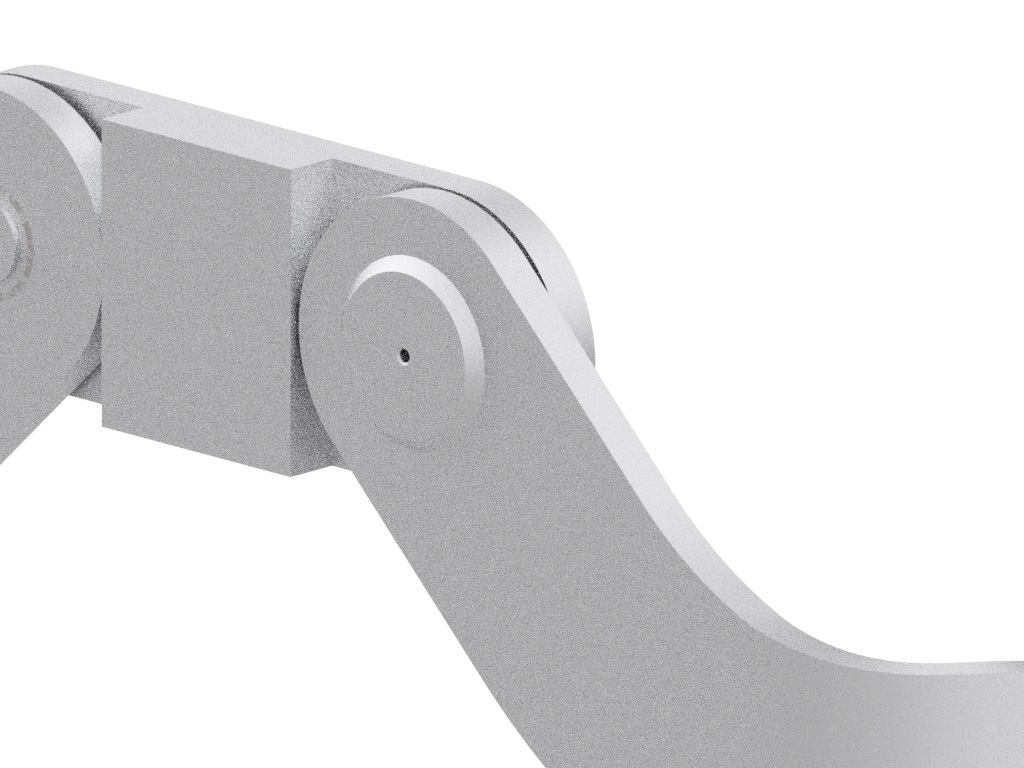
\includegraphics[width=0.4\textwidth]{Images/Junta_quadril_1.jpg}
      \caption{Hip abduction/adduction joint}
      \label{Junta Quadril 1}
   \end{figure}
   
Linked to these joint, a folded aluminum plate extends to the next hip joint.

\begin{figure}[thpb]
      \centering
      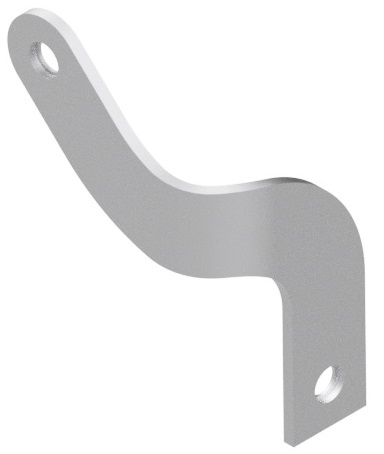
\includegraphics[width=0.4\textwidth]{Images/Chapa_quadril.jpg}
      \caption{Hip plate}
      \label{Chapa Quadril}
   \end{figure}
   
   The lateral joint allows for the flexion/extension degree of freedom of the thighs. This joint is also composed by a shaft supported by two ball bearings with a thrust washer between the two parts.
   
   \begin{figure}[thpb]
      \centering
      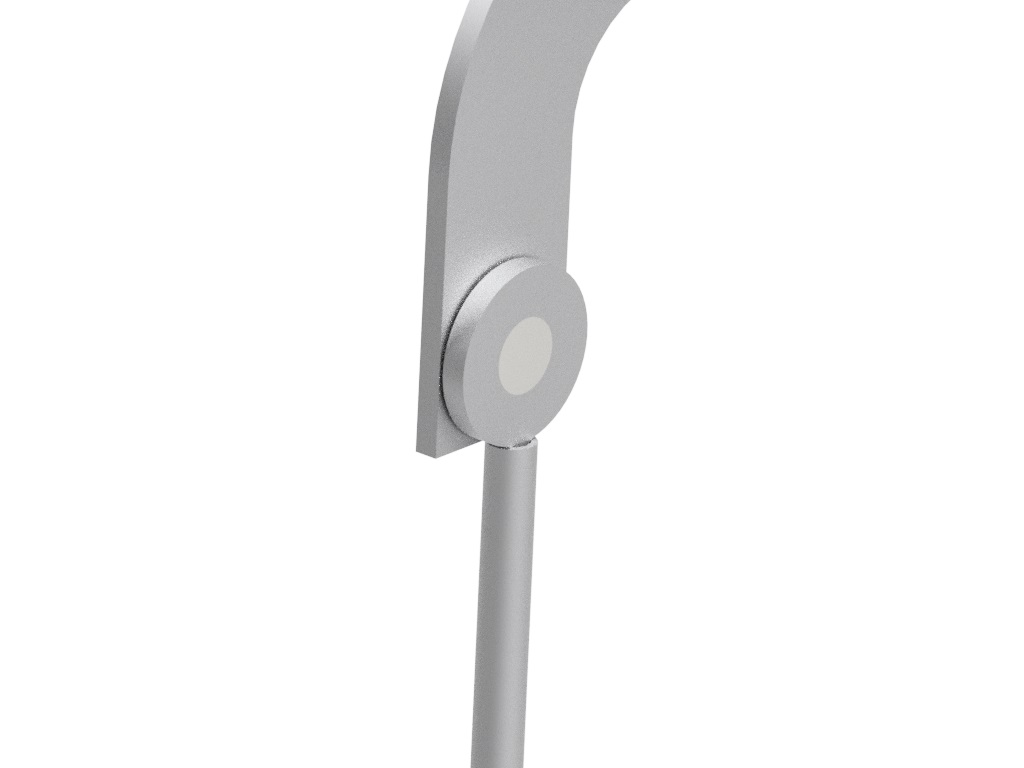
\includegraphics[width=0.5\textwidth]{Images/Junta_Quadril_2.jpg}
      \caption{Hip flexion/extension joint}
      \label{Junta Quadril 2}
   \end{figure}
   
   \subsubsection{Applied Forces}
   
   The weight of the user will be applied at the back support, attached to the hip base. For design purposes, the maximum user weight will be 1000 N. When walking with the exoskeleton, there is the possibility of the user tilting forward his upper body. The torque applied to the hip base due to this misalignment between the upper body and the base is considered as a 25 Nm torque. The torque applied at the joints is equal to 2000 N that is the maximum torque applied by the motors to the joints.
   
      \begin{figure}[thpb]
      \centering
      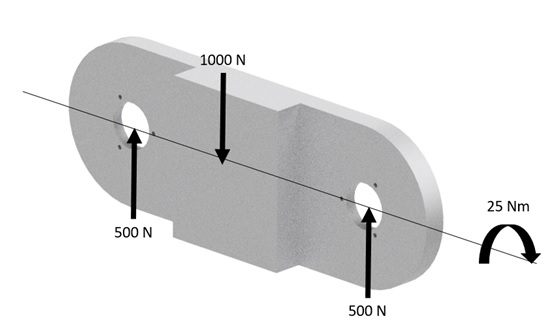
\includegraphics[width=0.4\textwidth]{Images/base_forcas.jpg}
      \caption{Acting forces on the base}
      \label{base forcas}
   \end{figure}
   
   \begin{figure}[b]
      \centering
      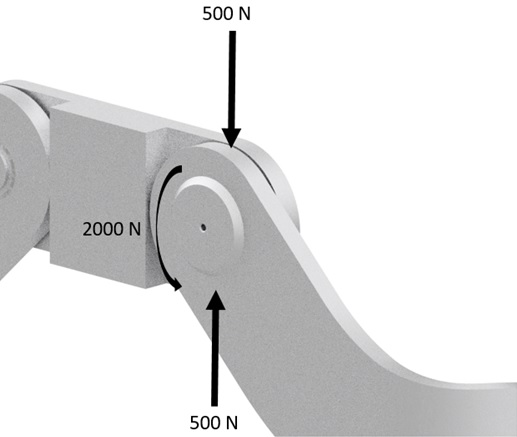
\includegraphics[width=0.4\textwidth]{Images/junta_quadril_1_forcas.jpg}
      \caption{Acting forces on the abduction/adduction joint}
      \label{junta quadril 1 forcas}
   \end{figure}
   

   
   \subsubsection{Materials}
   
   Aluminum was chosen for the structural plates as well as for the joints due to its low weight and high resistance/weight coefficient.
   
   The shafts will be constituted of steel, since they will support high loads. Because of its low dimensions, it is not critical the usage of low weight materials.
   
      \begin{figure}[thpb]
      \centering
      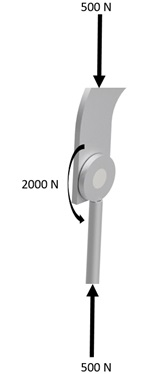
\includegraphics[scale=0.7]{Images/junta_quadril_2_forcas.jpg}
      \caption{Acting forces on the flexion/extension joint}
      \label{junta quadril 2 forcas}
   \end{figure}
   
   For the coupling of the shafts, ball bearings will be used so that the joints can rotate with low friction coefficient, as well as being capable of enduring the high loads applied. The chosen ball bearings were DIN 652 SKF with 2 RS1.
   
   To avoid interference between the two parts of the joints, a Permaglide\textsuperscript{\textregistered} thrust washer model PAW 26 will be used. This thrust washer has the necessary resistance to withstand the applied loads. Also, it is low weight and easier to assemble compared to axial bearings.
   
   The cover attached to the shaft will be made of aluminum.
   
   \bigskip
   
   \subsubsection{Calculations and simulations}
   
   Permaglide\textsuperscript{\textregistered} PAW 26 Thrust Washer:
   
   Torque at the hip due to the misalignment between the upper body and the rotation axis of the hip is considered as a 25 Nm torque. This torque will be supported by the thrust washer. That way:
   
   \begin{equation}
   M = 2\cdot F\cdot\frac{\frac{D_e}{2}+\frac{D_i}{2}}{2}
   \end{equation}
   
   \begin{equation}
   A = \frac{\frac{\pi}{4}(D_e^2-D_i^2)}{2}
   \end{equation}
   
   \begin{equation}
   \sigma = \frac{F}{A}
   \end{equation}
   
   Where M is the torque applied to the hip, F is the reaction force in the thrust washer and cover of the joint, $D_e$ and $D_i$ are the external and internal diameter of the thrust washer, respectively, A is the thrust washer area that will support the load and $\sigma$ is the load.
   
   Resulting in:
   
   $$\sigma \cong 1.5 MPa < \sigma_{crit}$$
   
   Therefore, the PAW 26 thrust washer is suitable to be used.
   
   DIN 625 SKF with 2 RS1 (SKF 61902-2RS1) ball bearing:
   
   Chosen through the SKF\textsuperscript{TM} bearing selection tool, for a load equal to 500 N and lifespan of 10000 hours. The tool can be found at: http://www.skf.com/group/knowledge-centre/engineering-tools/skfbearingselect.html
   
   All components were numerically simulated at the Autodesk\textsuperscript{TM} Inventor 2017 software. 
   
   \begin{figure}[thpb]
      \centering
      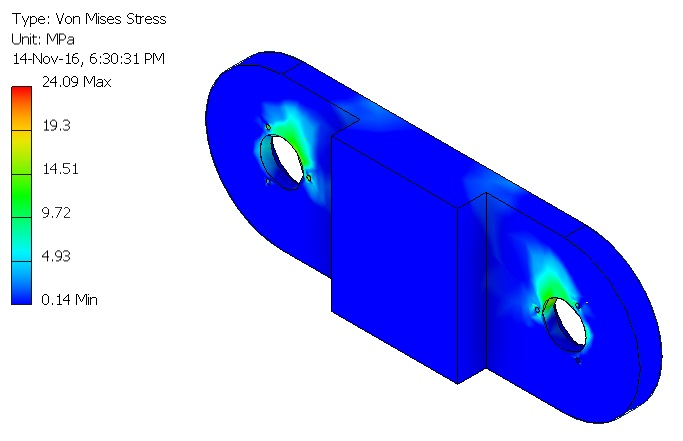
\includegraphics[scale=0.6]{Images/Simulacao_Base.jpg}
      \caption{Numerical simulation of the base}
      \label{simulacao base}
   \end{figure}
   
   \begin{figure}[thpb]
      \centering
      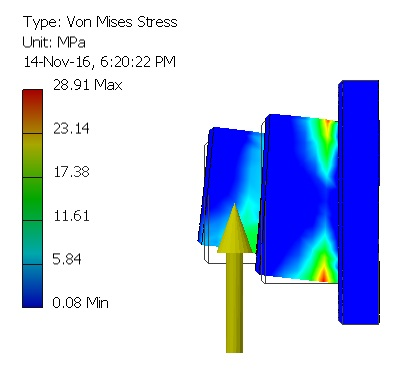
\includegraphics[scale=0.8]{Images/Simulacao_eixo.jpg}
      \caption{Numerical simulation of the joint shafts}
      \label{simulacao eixo}
   \end{figure}
   
   \begin{figure}[thpb]
      \centering
      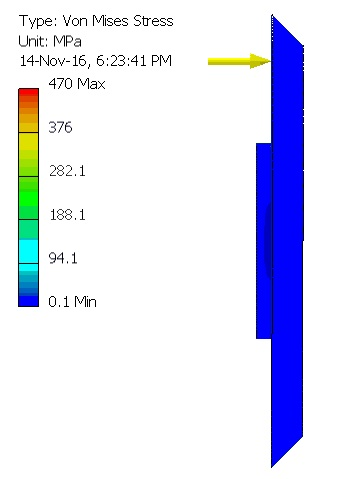
\includegraphics[scale=0.6]{Images/Simulacao_tampa.jpg}
      \caption{Numerical simulation of the cover}
      \label{simulacao tampa}
   \end{figure}
   
   \subsection{Knee}
   
   \subsubsection{Description}
   
   Each knee will have only one degree of freedom, aligned to the flexion/extension joint of the user. It is constituted of the following parts:
   
   A bar that extends from the flexion/extension joint of the hip to the knee joint. This bar stays parallel to the user's thigh.
   
   \begin{figure}[thpb]
      \centering
      
      \begin{subfigure}[b]{0.45\textwidth}
      	\centering
      	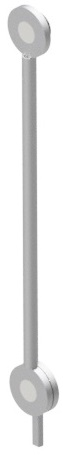
\includegraphics[height=0.3\textheight]{Images/Barra_Coxa.jpg}
      	\caption{Thigh}
      	\label{barra coxa}  
      \end{subfigure}
      ~
      \begin{subfigure}[b]{0.45\textwidth}
      	\centering
      	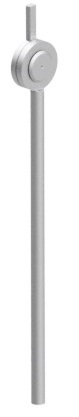
\includegraphics[height=0.3\textheight]{Images/Canela.jpg}
     	\caption{Leg}
     	\label{barra canela}
      \end{subfigure}
      \caption{Thigh and leg bars}
      
   \end{figure}
   
   Attached to the thigh bar, a rotation joint allows the flexion/extension movement of the mechanism. At this joint a shaft supported by two ball bearings will be used. Between the two parts of the joint a low friction coefficient thrust washer is positioned to support the axial forces and allow for smooth sliding between the parts. Another thrust washer is positioned at the external part of the joint, along with a metallic cover, to support the axial forces.
   
   \begin{figure}[thpb]
      \centering
      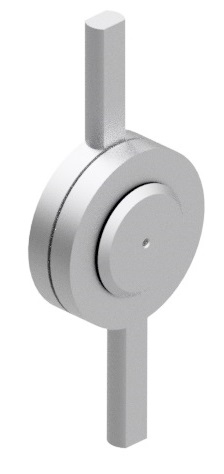
\includegraphics[scale=0.5]{Images/Junta_Joelho.jpg}
      \caption{Knee flexion/extension joint}
      \label{junta joelho}
   \end{figure}
   
   Attached to this joint, another metallic bar extends to the ankle.
   
   
   \subsubsection{Applied forces}
   
   The forces applied at the knee joint are the torque that the motor applies at the joint and the weight of the user and exoskeleton. 
   
   \begin{figure}[thpb]
      \centering
      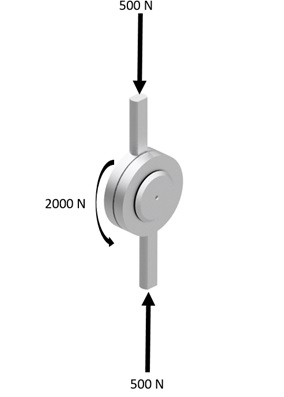
\includegraphics[scale=0.5]{Images/joelho_forcas.jpg}
      \caption{Forces applied to the knee joint}
      \label{joelho forcas}
   \end{figure}
   
   \subsubsection{Materials}
   
   Aluminum is the metal constituting the joints. This material was chosen for its low weight and high resistance/weight coefficient.
   
   For the bars, steel bars will be used for its high resistance and easy acquisition.
   
   For the same reasons stated at the hip, the shafts will be made of steel.
   
   Like before, DIN 625 SKF with 2 RS1 ball bearings and PAW 26 Permaglide\textsuperscript{\textregistered} thrust washers will be used.
   
   \subsubsection{Calculations and simulations}
   
   \begin{figure}[thpb]
      \centering
      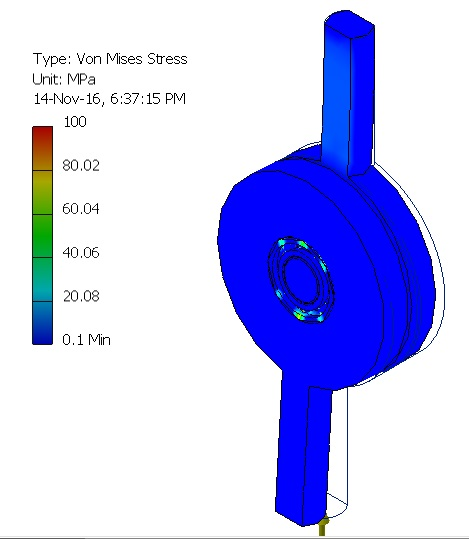
\includegraphics[scale=0.5]{Images/Simulacao_Joelho.jpg}
      \caption{Numerical simulation of the knee joint}
      \label{simulacao joelho}
   \end{figure}
   


   \chapter{Upper Limb Exoskeleton With One Degree of Freedom}
   
   \label{ch:ulexo}
   
   This chapter briefly describes an upper limb exoskeleton with one degree of freedom already available at the Biomechatronics laboratory. A more extensive description of this system can be found at \cite{Sommer2015}.
   
   \section{Mechanical}
   
   \subsection{Structure}
   
   The exoskeleton structure is made of aluminum bars. The aluminum structure is attached to a Power Window Lifter steel mechanism.
   
   The user's arm is placed at the aluminum structure and held firmly through the use of rubber straps.
   
   \begin{figure}[thpb]
      \centering
      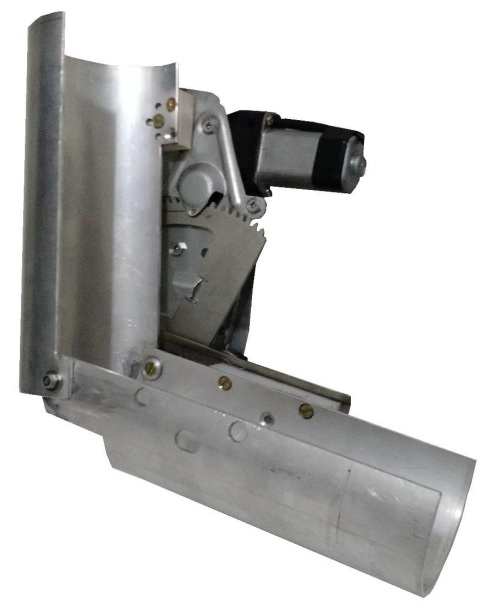
\includegraphics[scale=0.5]{Images/Exoskeleton.jpg}
      \caption{Upper limb exoskeleton with one degree of freedom \cite{Sommer2015}}
      \label{exoskeleton}
   \end{figure}
   
   \subsection{Actuator}
   
   The actuator of the exoskeleton is composed by a Mabuchi JC-578VA-4720 DC motor and a Power Window Lifter mechanism.
   
   This DC Motor was chosen because of its high power-to-weight ratio, low dimensions and low price.
   
   In order to increase the motor torque, the DC motor is attached to a modified Power Window Lifter, a mechanism with gear coupling with a reduction factor of 10:1.
   
   \begin{figure}[thpb]
      \centering
      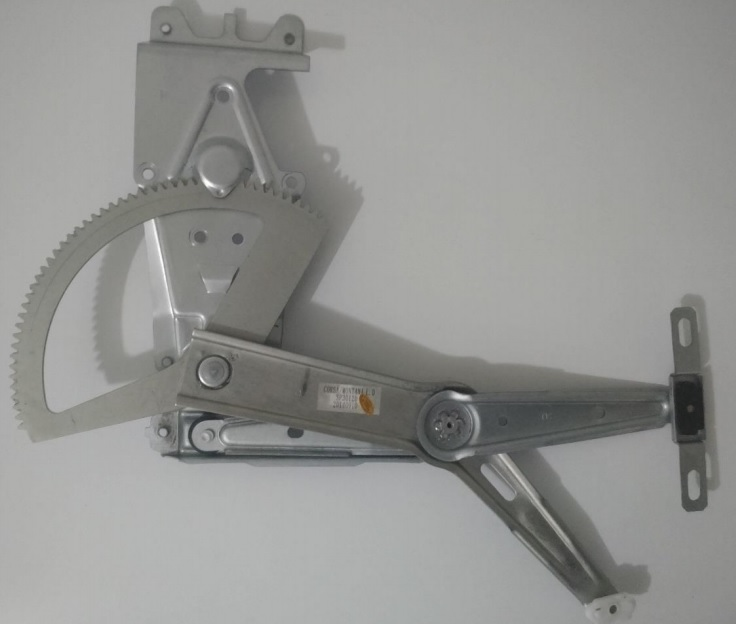
\includegraphics[scale=0.5]{Images/PowerWindowLifter.jpg}
      \caption{Power Window Lifter \cite{Sommer2015}}
      \label{PowerWindowLifter}
   \end{figure}
   
   \section{Electronics}
   
   The electronics system of the exoskeleton is composed of the following parts: An sEMG sensor, that acquires the sEMG signal of the target muscle; a microprocessor to process the analog sEMG signal, apply the control logic and output a PWM signal; a motor driver that receives the PWM signal as input and outputs the necessary power to drive the DC motor.
   
   \begin{figure}[thpb]
      \centering
      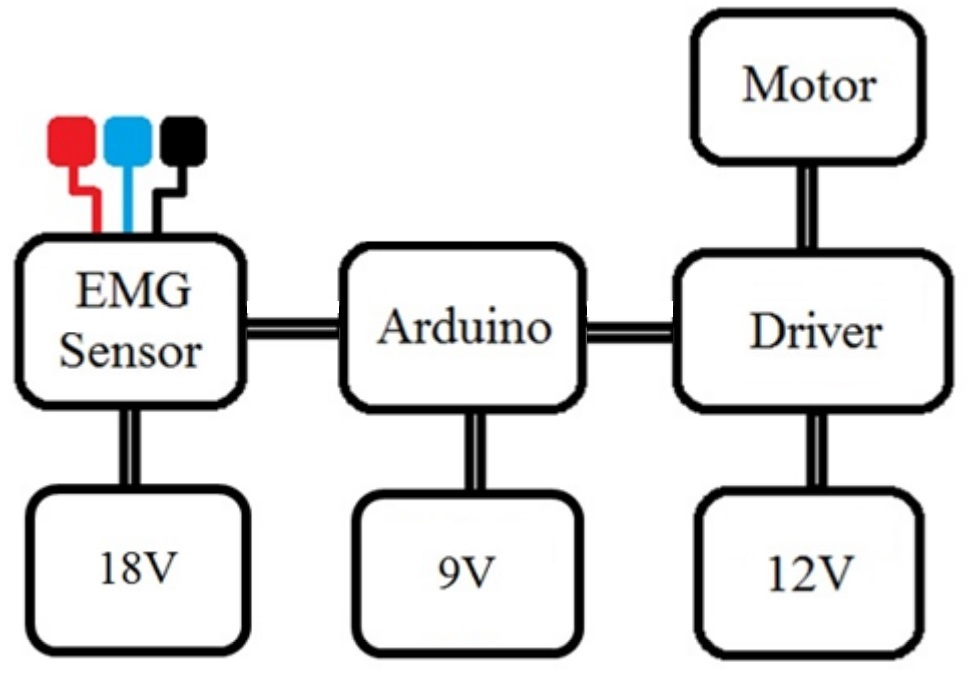
\includegraphics[scale=0.5]{Images/ElectronicSchematic.jpg}
      \caption{Schematic of the electronics \cite{Sommer2015}}
      \label{ElectronicSchematic}
   \end{figure}
   
   \subsection{EMG Sensor}
   
   The EMG Sensor is a SparkFun Muscle Sensor V3. 
   
   Three electrodes are attached to this sensor: Two electrodes are placed at the target muscle and measure the difference of electrical activity and one is placed at an electrically neutral region of the body, like a bony area, and serves as the ground signal.
   
   The signal from the electrodes is differentially amplified in the AD8221 amplifier; then, the signal is amplified twice by TL084 operational amplifiers; the signal is rectified using 1N4148 diodes; the rectified signal is attenuated by a filter; at last, the signal is amplified with an adjustable gain.
   
   The Sensor output is sent directly to the microprocessor. 
   
%    \begin{figure}[thpb]
%       \centering
%       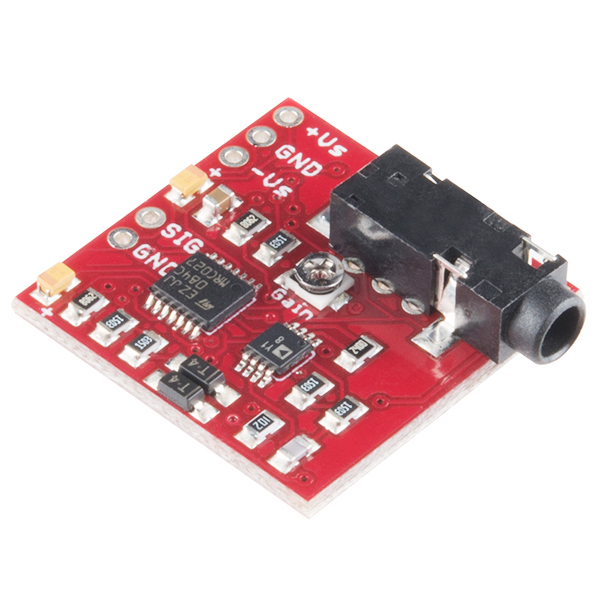
\includegraphics[height=0.3\textheight]{Images/MuscleSensorV3.jpg}
%       \caption{Muscle Sensor V3 \cite{musclesensorv3}}
%       \label{MuscleSensorV3}
%    \end{figure}
   
   \subsection{Microprocessor}
   
   The microprocessor is an Arduino UNO. It was chosen for its low cost, ease-of-use, extensive available documentation and easy communication to the Muscle Sensor V3. It has a built-in Analog/Digital converter and is capable of emitting PWM signals. Also, it is possible to connect more sensors to this microprocessor, for future adaptations of the exoskeleton.  

   
   \subsection{Driver}
   
   The DC motor demands electrical currents up to 24A. Motor Drivers for 12V, 24A DC motors are expensive. For this reason, a motor driver was designed for the specific use on this exoskeleton.
   
   The driver has two inputs (clockwise rotation and counter-clockwise rotation) that receives the PWM signal from the microprocessor for the desired direction of motion. There are two outputs that are connected to each one of the motor electrical terminals.
   
%    \begin{figure}[thpb]
%       \centering
%       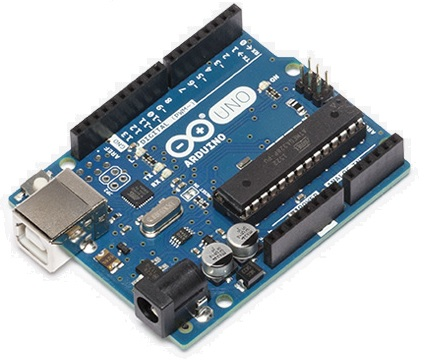
\includegraphics[height=0.3\textheight]{Images/arduino.jpg}
%       \caption{Arduino UNO. Image adapted from \cite{arduino}}
%       \label{arduino}
%    \end{figure}
   
   The driver is composed of a H-Bridge of MOSFETs. The chosen components were IRF4905 for P channel and IRLB3813 for N channel. The gate of the P channel MOSFET is powered by a TIP122 transistor.
   
   To avoid the situation where every MOSFET of the H-Bridge is activated at the same time, which would cause a short circuit between the poles of the battery, a protection circuit was implemented. The protection circuit is composed of 74LS08 AND gates and 74LS04 NOT gates. In case both the inputs are powered, no signal reaches the gates of transistors, protecting the circuit.
   
      

\chapter{ModExo}
\label{ch:ModExo}

\section{Mechanical}
\subsection{Structure}

\subsection{Actuator}

\section{Electronics}
\subsection{Sensors}

\subsection{Driver}

\subsection{Microprocessor}

\mypart{Control Design and Testing}{In this part, control methods for the EMG and mechanical control are proposed, designed, implemented and evaluated to determine which one is better suited for controlling an exoskeleton.}

\chapter{Impedance and Sliding Mode Control of a One Degree of Freedom Exoskeleton}

\section{Exoskeleton Model}

\subsection{Exoskeleton}

In this study, we will use the upper limb exoskeleton described at chapter \ref{ch:ulexo}. It has one degree of freedom on the elbow joint, actuated by a DC motor with a Power Window Lifter gear transmission. The motor used is a 12V Mabuchi 578VA. The transmission has a 10:1 reduction ratio. The structure of the exoskeleton is constructed on aluminum. 

The exoskeleton is illustrated in figure \ref{exoskeleton system}. When the user tries to flex his arm, an electrical voltage can be recorded from the electrodes placed on the skin next to the biceps brachii. The SparkFun Muscle Sensor V3 was used to measure the EMG. It acquires the biceps muscle voltage, rectifies, low-pass filters  and amplifies the signal. This signal is sent to a microprocessor (in this case the ATmega328P), that makes the analog-to-digital conversion and applies a moving average filter. Finally the voltage signal is transformed into a desired joint angle. Equation \ref{eq:voltage_angle} shows the equation that gives the desired joint angle as a function of the EMG sensor voltage. A linear relationship between the angular position and the measured voltage was chosen. The equation was defined by measuring the lowest and highest voltage level acquired from the biceps muscle and linearly scaling it to the minimum angle of 0 and maximum angle of \(\frac{\pi}{2}\). It is important to note that the voltage from the EMG sensor is never zero. Even at a relaxed position, the sensor measures a residual voltage level.

\begin{equation}
\label{eq:voltage_angle}
\theta_d = -0.29 + 0.582 * V_{emg}
\end{equation}

\begin{figure}[thpb]
      \centering
      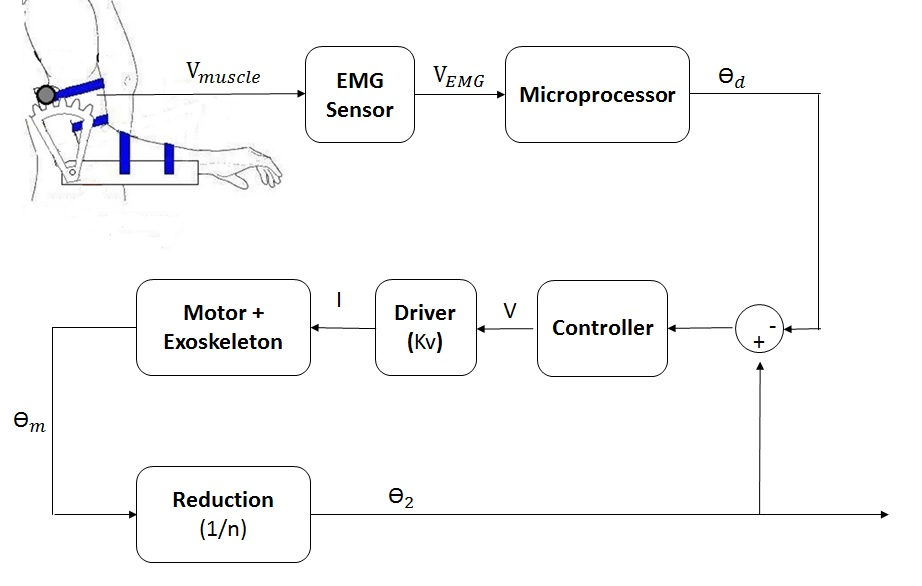
\includegraphics[scale=0.5]{Images/Exoskeleton_System.jpg}
      \caption{Diagram showing the exoskeleton block diagram control}
      \label{exoskeleton system}
   \end{figure}
   
   With the desired joint angle the PWM magnitude sent to the motor driver is calculated with a control logic in order to control the motor that actuates the exoskeleton. This control logic will be further studied in the next section. The motor driver input is the PWM voltage and its output is an electrical current. Equation \ref{eq:current} shows the relationship between PWM voltage and motor current:
   
   \begin{equation}
\label{eq:current}
I = K_v*V
\end{equation}

Where \(K_v = 1.42\) is the driver gain, V is the voltage applied to the driver and I is the output current of the driver.

The output electrical current from the driver goes to the motor, actuating the exoskeleton and consequently moving the user’s forearm.

\subsection{Modeling}

Even though the exoskeleton has only one degree of freedom on the elbow joint, the user's shoulder angle should be considered because it influences the forces applied to the exoskeleton and the arm. The exoskeleton can be modeled as two segments: the upper arm (between shoulder and elbow) and the forearm (between elbow and wrist).

\begin{figure}[thpb]
      \centering
      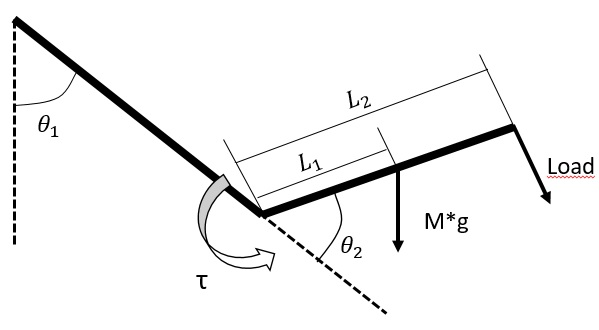
\includegraphics[scale=0.5]{Images/DCL_exoesqueleto.jpg}
      \caption{Free body diagram of the exoskeleton}
      \label{exoskeleton fbd}
   \end{figure}

Figure \ref{exoskeleton fbd} shows the exoskeleton free body diagram, where the upper arm is considered to be fixed at a given angle \(\theta_1\), \(\theta_2\) is the angle between the upper arm and the forearm with a motion range between 0 and \(\frac{\pi}{2}\) rad, \(\tau\) is the torque applied by the motor, the Load has a range between 0 and 100N, M is the sum of the human forearm and exoskeleton forearm masses that equals 2.14 kg, \(L_1\) is the distance between the elbow center and the forearm center of mass (0.12m), \(L_2\) is the length of the forearm (0.22m), \(J_e\) is the forearm moment of inertia \(5.6 \cdot 10^{-3}  kg\cdot m^2\).

Equation \ref{eq:coupled exo motor} shows the dynamics of the exoskeleton:

\begin{equation}
\label{eq:coupled exo motor}
\left(\frac{J_e}{n}+J_m\right)\cdot \ddot{\theta}_m+B \cdot \dot{\theta}_m = \tau + \frac{-L_2 \cdot Load - L_1 \cdot M \cdot g \cdot sin\left(\frac{\theta_m}{n}+\theta_1\right)}{n}
\end{equation}
   
   Equation \ref{eq:motor torque} gives the relation between motor input current and output torque:
   
   \begin{equation}
\label{eq:motor torque}
\tau = k_m \cdot I
\end{equation}

Using equations \ref{eq:current}, \ref{eq:coupled exo motor} and \ref{eq:motor torque} gives the exoskeleton and human dynamics:

\begin{equation}
\label{eq:plant dynamics}
\left(\frac{J_e}{n}+J_m\right)\cdot \ddot{\theta}_m+B \cdot \dot{\theta}_m = K_m \cdot K_v \cdot V +\frac{-L_2 \cdot Load - L_1 \cdot M \cdot g \cdot sin\left(\frac{\theta_m}{n}+\theta_1\right)}{n} 
\end{equation}

Where \(\theta_m\) is the angle of the shaft of the motor, \(J_m = 6 \cdot 10^{-5} kg \cdot m^2\) is the inertia of the motor, B = 1.2732 is the damping coefficient of the motor, n = 10 is the reduction factor and \(K_m = 0.533\) is the electrical current gain of the motor.

\section{Control}

\subsection{General Characteristics}

The action control will be the voltage V applied to the driver of the motor. 
The load applied to the exoskeleton can vary from 0N to 100N. In this way the user will be able to manipulate different objects without changing the control parameters in a short time span. The controller goal is to control the exoskeleton position while maintaining safety and confort. The range of motion of the elbow joint is from 0 to \(\frac{\pi}{2}\) rad while the maximum angular velocity must be around \(\frac{\pi}{4}\) rad/s. There must be no overshoot on the movement.

\subsection{Impedance Control}

The first law will be based on impedance control. Impedance control imposes a dynamic behavior to the interaction between the target system and the environment, usually a mass-spring-damper system.	
Impedance control is suited for tasks that require contact forces without an accurate control of the end-effector position (e.g. grabing an object). That is especially important in biomechanical applications since the human arm is capable of doing delicate tasks without a profound knowledge of necessary forces to be applied to the target objects. 
One drawback is that whenever an external force is applied on the system the final position of the end-effector will not necessarily be the desired one, instead it controls a combination of force and position. The chosen stiffness for the dynamic system will regulate this trade-off between contact force and position accuracy.

\subsection{Impedance Control Design}

The system dynamics, (equation \ref{eq:plant dynamics}), can be rewritten as follows:


\begin{equation}
\begin{split}
\label{eq:rewritten plant}
\ddot{\theta}_m = \frac{-B \cdot \dot{\theta}_m + \frac{-L_2 \cdot Load - L_1 \cdot M \cdot g \cdot sin (\frac{\theta_m}{n}+\theta_1 )}{n} + K_v \cdot K_m \cdot V }{\frac{J_e}{n}+J_m}
\end{split}
\end{equation}

Equation \ref{eq:rewritten plant} can be organized in the form:

\begin{equation}
\label{eq:reorg}
\ddot{\theta}_m = f + bu
\end{equation}

Where:

\begin{equation}
\label{eq:f}
f = \frac{-B \cdot \dot{\theta}_m + \frac{-L_2 \cdot Load - L_1 \cdot M \cdot g \cdot sin \left(\frac{\theta_m}{n}+\theta_1 \right)}{n}}{\frac{J_e}{n}+J_m}
\end{equation}

\begin{equation}
\label{eq:b}
b = \frac{K_v \cdot K_m}{\frac{J_e}{n}+J_m}
\end{equation}

\begin{equation}
\label{eq:u}
u = V
\end{equation}

The desired closed loop dynamics are:

\begin{equation}
\label{eq:desired}
M_d \cdot (\ddot{\theta}_m-\ddot{\theta}_d) + B_d \cdot (\dot{\theta}_m - \dot{\theta}_d) + K_d \cdot (\theta_m - \theta_d) = -F
\end{equation}

Where \(M_d\) is the desired inertia, \(B_d\) is the desired damping, \(K_d\) is the desired stiffness, \(\theta_d\) is desired position and 

\begin{equation}
\label{eq:F}
F = \frac{L_2 \cdot Load}{n}
\end{equation}

This characterizes a mass-spring-damper dynamics that will be imposed to the system by the controller.

By substituting equation \ref{eq:desired} in equation \ref{eq:reorg} and rearranging, one gets:

\begin{equation}
\label{eq:subs1}
u = b^{-1} \left(-f+ \frac{M_d \cdot \ddot{\theta}_d-B_d \cdot (\dot{\theta}_m-\dot{\theta}_d)-K_d \cdot (\theta_m-\theta_d)-F}{M_d}\right)
\end{equation}

Equation \ref{eq:subs1} gives the control law for the system, that can be expressed as (using \ref{eq:rewritten plant} - \ref{eq:F})

\begin{equation}
\begin{split}
\label{eq:inpedance law}
V = {} & \frac{1}{K_v \cdot K_m} (B \cdot \dot{\theta}_m + \frac{L_2 \cdot Load}{n} + \frac{L_1 \cdot M \cdot g \cdot sin(\frac{\theta_m}{n}+\theta_1)}{n} + \\ 
& (\frac{J_e}{n}+J_m)(M_d \cdot \ddot{\theta}_d - B_d(\dot{\theta}_m-\dot{\theta}_d)-K_d(\theta_m-\theta_d)-\frac{L_2 \cdot Load}{n})\cdot \frac{1}{M_d})
\end{split}
\end{equation}

This control law, as it is presented, cancels the nonlinearities of the system and imposes the desired dynamic  system behavior to the exoskeleton.

\subsection{Sliding Mode Control Design}

The second applied control law will be the Sliding Mode control. The system dynamics are the same as shown in equation \ref{eq:coupled exo motor}

The desired sliding surface is:

\begin{equation}
\label{eq:SM}
s = \dot{\theta}_m - \dot{\theta}_{d} + \lambda \cdot (\theta_m-\theta_{d})
\end{equation}

The control signal is u and, to achieve the desired controlled dynamics of the system, its value is as follows:

\begin{equation}
\label{eq:uSM}
u = \hat{b}^{-1}\left(-\hat{f}+\ddot{\theta}_{d} -\lambda \cdot (\theta_m-\theta_{d})-K\cdot sat\left(\frac{s}{\phi}\right)\right)
\end{equation}

Where:

\begin{equation}
\label{eq:bSM}
\hat{b} = \frac{K_v \cdot K_m}{\frac{J_e}{n}+\hat{J}_m}
\end{equation}

\begin{equation}
\label{eq:fSM}
\hat{f} = \frac{-B \cdot \dot{\theta}_m + \frac{-L_2 \cdot \hat{Load} - L_1 \cdot M \cdot g \cdot sin(\frac{\theta_m}{n}+\theta_1)}{n}}{\frac{J_e}{n}+\hat{J}_m}
\end{equation}

\(\hat{J_m}\) is the motor inertia with measuring error and \(\hat{Load}\) is the external load applied to the exoskeleton with measuring error.

This way, when in closed loop, the system acquires the following dynamics:

\begin{equation}
\label{eq:CLSM}
\frac{ds}{dt} = (\ddot{\theta}_m-\ddot{\theta}_{d})+\lambda \cdot (\dot{\theta}_m-\dot{\theta}_{d})
\end{equation}

That is,

\begin{equation}
\begin{split}
\label{eq:CLSM}
\frac{ds}{dt} = {} & f + b \cdot \hat{b}^{-1} \cdot (-\hat{f}) + b \cdot \hat{b}^{-1} \cdot (\ddot{\theta}_{d} - \lambda \cdot (\theta_m - \theta_{d}) +  \\
& - b \cdot \hat{b}^{-1} \cdot K \cdot sat(\frac{s}{\phi})-\ddot{\theta_m} + \lambda \cdot (\dot{\theta}_m-\dot{\theta}_{d}))
\end{split}
\end{equation}

To guarantee convergence the control must satisfy a sliding condition:

\begin{equation}
\label{eq:condition}
\frac{1}{2}\frac{ds^2}{dt} \leq -\eta \cdot |s|
\end{equation}

Equation \ref{eq:condition}, using \ref{eq:CLSM}:

\begin{equation}
\label{eq:K}
K \leq \beta \cdot (\eta + F) + (\beta -1) \cdot |\hat{u}|
\end{equation}

Where,
\begin{equation}
\label{eq:beta}
\beta = \sqrt{\frac{b_{max}}{b_{min}}}
\end{equation}

\begin{equation}
\label{eq:Fsm}
F > |f-\hat{f}|
\end{equation}

\begin{equation}
\label{eq:uhat}
\hat{u} = -\hat{f} + \ddot{\theta}_{d}-\lambda \cdot (\theta_m - \theta_{d})
\end{equation}

\section{Results}

\subsection{Impedance Control}

Choosing \(M_d = 1 kg \cdot m^2, B_d = 4 N \cdot m \cdot s, K = 4.5 N \cdot m\) and \(\theta_d = 1 rad\) gives \(\omega_n = \frac{2\pi}{8}\) rad/s the natural frequency of the system, \(t_{0-90\%} = 2.4 s\) the time the system takes to reach 90\% of the final position and \(\zeta > 1\) the damping factor, since there must be no overshoot.

Figures \ref{posicao0} and \ref{posicao100} show the results of a simulation where \(\theta_d = 1 rad\) and external load = 0 and 100N, respectively.

\begin{figure}[thpb]
      \centering
      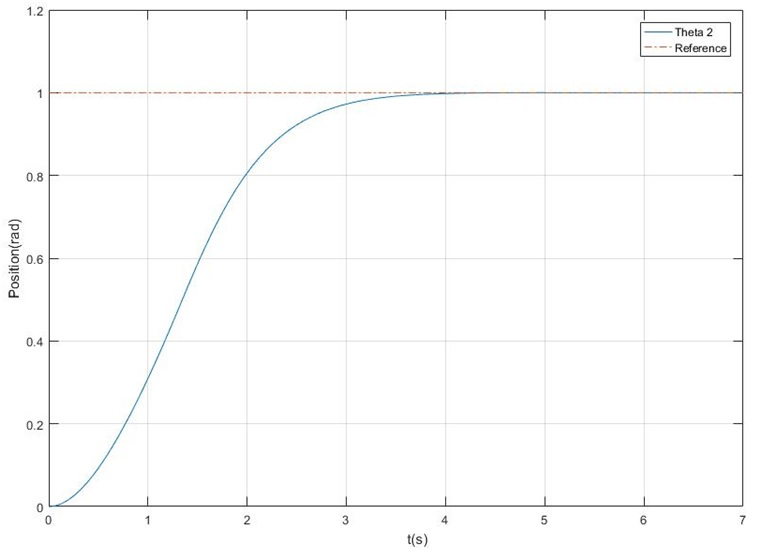
\includegraphics[scale=0.5]{Images/posicao_load_0_paper.jpg}
      \caption{Position \(\theta_2\) versus time for an external load = 0}
      \label{posicao0}
   \end{figure}
   
   \begin{figure}[thpb]
      \centering
      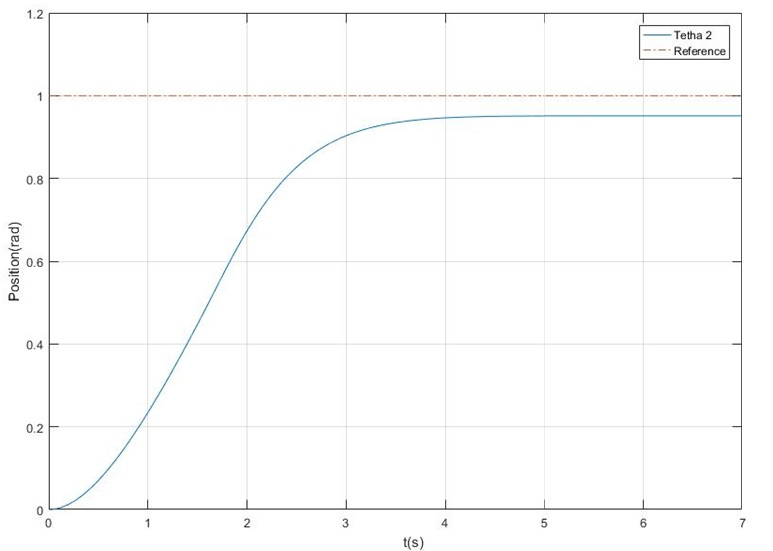
\includegraphics[scale=0.5]{Images/posicao_load_100_paper.jpg}
      \caption{Position \(\theta_2\) versus time for an external load = 100 N}
      \label{posicao100}
   \end{figure}

\subsection{Sliding Mode Control}

Considering the measured load with 30\% error and the measured motor inertia with 20\% error, that is, \(\hat{Load} = 130N\) and \(\hat{J}_m = 7.2 \cdot 10^{-5} kg \cdot m^2\), resulting in \(\beta = 1.04\), the system was simulated with the following parameters: \(\eta = 5, \lambda = 1\) and \(\phi = 10\) and the results for the position and the sliding surface can be found in figures \ref{posicaoSliding} and \ref{slidingSurface}, respectively.

\begin{figure}[thpb]
      \centering
      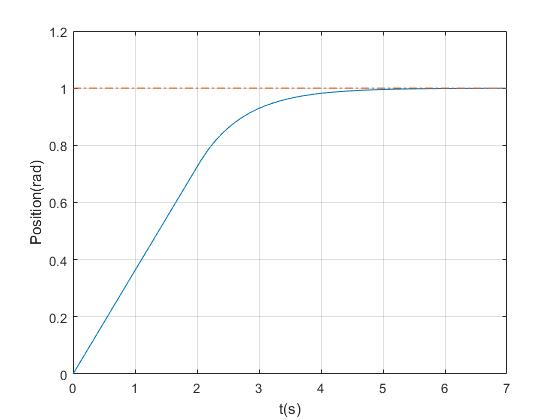
\includegraphics[scale=0.5]{Images/Sliding_mode_position.jpg}
      \caption{Position \(\theta_2\) versus time}
      \label{posicaoSliding}
   \end{figure}
   
   \begin{figure}[thpb]
      \centering
      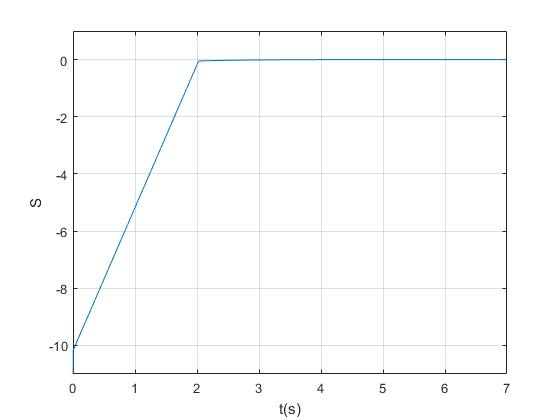
\includegraphics[scale=0.5]{Images/Sliding_mode_S.jpg}
      \caption{Sliding surface versus time}
      \label{slidingSurface}
   \end{figure}

\section{Conclusions}

Both control approaches has advantages and drawbacks. The impedance control cannot reach a desired position with utmost accuracy since the external load, by definition, will take the system out of its desired final position and the system parameters must be precisely measured in order to guarantee accurate desired dynamics. On the other hand, precise activities can be achieved without a deep knowledge of the environment, the system acquires familiar characteristics in the form of a mass-spring-dampener system and it is safer for the user since the controller changes the position of the system when an excessive external load is detected. The sliding mode control can achieve great precision and accuracy of desired position and trajectory and does not require a precise measurement of the system characteristics.

Depending on the application each one of these control methods is more appropriated. In the case of a wearable exoskeleton, the impedance control is a more suitable control method, since it offers a dynamic behavior close to that of a human limb and is safer for the user. To control an external robotic arm, the sliding mode control can be used since it will cause no harm to the user and is capable of performing actions with higher accuracy.

\chapter{General EMG-driven controller characteristics}

The main focus of this present work is to design a control method that allows the user to control an exoskeleton. 

The ideal control method would be one that requires no prior training. The user would be capable of controlling the mechanism as easily as he can control his own limb. Of course this is an ideal scenario and, as stated in many previous studies already cited in this work, we are still far from understanding the real dynamics of limbs, muscles and electromyography signals.

With those challenges in mind, how can we design a control that is capable of controlling a mechanical "limb-like" mechanism?

The first idea that comes to mind is to design a control method that mimics the physical characteristics of the human limb, that is, a biomimetic control. Biomimetics is the study of biological mechanisms and processes with the purpose of synthesizing similar products and behaviors by an artificial mechanism which mimics natural ones \cite{merriamWebster}. To achieve this biomimetic behavior, the model-based control method is proposed.

Many times for the control of machines, like cars, the control systems do not use biomimetic mechanisms. Instead, an easier mechanism or system is designed so that, with the proper training, the user is capable of controlling the machine even in complex activities. With that idea in focus, we can use the proportional EMG control.

As many prior studies have stated, the usage of hybrid methods can enhance the accuracy and ease-of-use of the controller. In this work, a control method using sEMG and force sensors will be applied.

For this work, these three control methods will be designed, applied to the mechanism and evaluated.














\chapter{Model-based EMG-driven Control}
\label{ch:ModelControl}

% Atualizar para novo texto presente nos artigos.

\section{Control Description}

The Model-Based control method utilizes a dynamic model of the body to predict the dynamic response according to the input given to the model.

There are basically three ways the dynamic model can be obtained: through mathematical model, system identification model and artificial intelligence model \cite{Anam2012988}.

For this work the chosen model is the system identification model.  The system identification method is often used because of the difficulty in precisely describe the dynamic model through mathematical equations. To do so, a set of inputs and outputs are measured through experiments and then an identification algorithm develops the relationship between the inputs and outputs of the system.

%Four modeling techniques were applied to determine which one better estimates the model which determines the elbow angle with EMG signals as input: ARX, ARMAX, ARIMAX and SS. The model that had the highest fitness value was the ARMAX model.

By using a dynamic model that mimics the user's limb dynamics, the exoskeleton will be capable of performing limb-like movements using the sEMG signals as input.

The main disadvantage of this control method is that, in order to develop the dynamic model, extensive experiments must be conducted on each subject to calculate his/her specific model parameters. Even a slight change in the electrode positioning on the subjects' skin can alter the results from the controller. This would require a calibration procedure every time the user wears the exoskeleton.

\section{Conducted experiment}

This section presents a method to estimate the elbow joint angle from surface electromyography (sEMG) measurements of biceps, triceps and brachioradialis. This estimation is of major importance for the design of human robot interfaces based on sEMG, for the modeling of the muscular system and for the design of bio-inspired mechanisms. However, the interpretation and processing of electromyography signals is challenging due to nonlinearities, unmodeled muscle dynamics noise and interferences. In order to determine an estimation model and a calibration procedure for the model parameters, a set of experiments were carried out with seven subjects. The experiments consisted of series of continuous (cyclical) and discrete elbow flexo-extensions. The sEMG data from the biceps brachii, triceps brachii and brachioradialis and the joint angle were recorded. After the model was selected, a second experiment was performed in order to validate the estimation procedure. The results show an effective model for the EMG-to-angle relation with great values for both correlation and mean-square-root error when compared to the measured angle data.

\subsection{Methods}
\subsubsection{Subjects and experimental setup}
Seven volunteers (age: 34.3 $\pm$ 14.7 years, height: 1.74 $\pm$ 0.1 m, weight: 67.9 $\pm$ 15.7 kg, 4 male, 3 female, all right-handed) with no known neuromuscular deficit participated in the experiments. Elbow joint angle along with the surface Electromyography (sEMG) of three right arm muscles, biceps brachii, triceps brachii and brachioradialis were recorded. 
sEMG was measured with 3 pairs of BTS FREEEMG 1000 \textsuperscript{\textregistered} electrodes with an electrode separation of 20mm with the electrode diameter being 4mm. A pair of electrodes was placed on the biceps and other pair on the triceps following the SENIAM guidelines \cite{SENIAM20170110}. To determine the electrode positions of the brachioradialis muscle, the subject was asked to apply force to flex the forearm while keeping it at \(90^{\circ}\). Then, the electrode was placed on the belly of the muscle and its respective pair placed distally at a 20mm following the muscle fiber direction. The sampling rate was of 1kHz with 16 bit resolution. The user interface was the BTS FREEEMG software. 

To measure the joint angle, a six degrees of freedom Inertial Measurement Unit (IMU, VN-100 from VectorNav\textsuperscript{\textregistered}), with \(0.01^{\circ}\) precision, was attached on the internal aspect of the forearm, located at two-thirds distance from the elbow to the wrist. The angle values were acquired with a rate of 100 samples per second. The data were collected with Matlab\textsuperscript{\textregistered} 

\subsubsection{Experimental Protocol}

\begin{figure}[thpb]
      \centering
      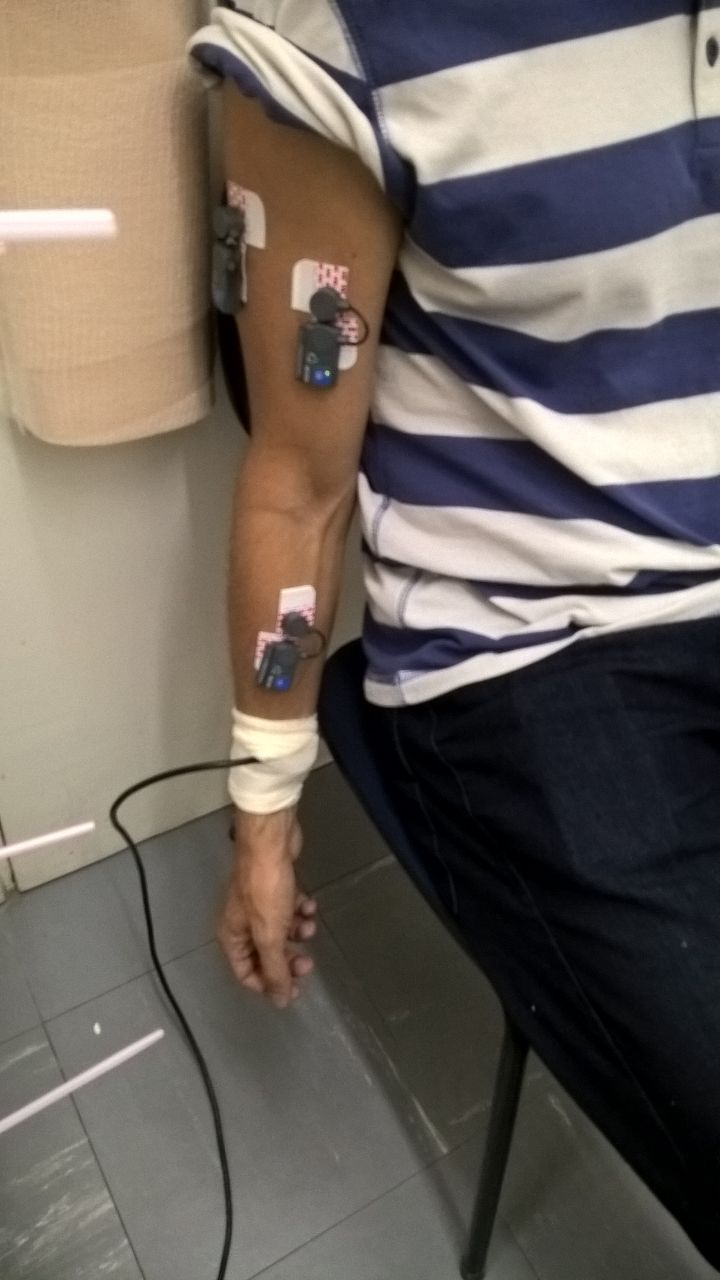
\includegraphics[scale=0.32]{Images/Experiment_Image.jpg}
      \caption{Experimental setup on a test subject}
      \label{Experimental Setup}
   \end{figure}

The subject sat on a chair, with the knees flexed at \(90^{\circ}\), the back perpendicular to the ground with the scapulas pressed against the wall. The back of the arm was leaning against a rubber support that was attached to the wall. This setup guaranteed that the subject was comfortable enough to perform repeated elbow flexions and extensions while maintaining the upper arm steady. 

The test protocol had three parts: The first one consisted of an isometric force test to obtain the Maximum Voluntary Contraction (MVC). The elbow of subject was kept in a fixed position at \(90^{\circ}\) and he/she was asked to apply the maximal possible force to flex the elbow. The subject was given a three minute interval before the next set.


In the second part, the subject was asked to perform five consecutive elbow flexion and extension movements from  \(50^{\circ}\) to \(140^{\circ}\) with a frequency of 0.5Hz. To help the subject reach the correct target angles a template was attached to the wall parallel to the subject, to provide visual guidance. To achieve the desired movement speed a metronome was set at the speed of 60 bpm so that the subject could synchronize the movements with the sound of the metronome.    

   The subject was given a minute of rest before the third part of the experiments. In this part the subject was asked to make an elbow flexion for 1s, then hold his forearm at \(140^{\circ}\) for 1 second, then a 1 second extension movement and then hold his forearm at \(50^{\circ}\) for another second. This movement should be repeated five times. Another one minute resting time was given to the subject.
Both of the continuous and interval tests were repeated with 1.5kg and 3kg extra weight placed at the subject's hand.

No subjects reported fatigue during the experiment.

The test was repeated in a different day, on all test subjects to further analyze the repeatability of the model proposed in this work.

All the data from the tests were transferred to Matlab\textsuperscript{\textregistered} for further analysis and processing.



\subsubsection{Experimental Data Processing}

The EMG data were processed as follows. Further explanations can be found on the literature \cite{Rose20161112}\cite{hayashibe:lirmm-00429594}
\begin{enumerate}
\item high-pass filtering of the EMG data, using a 2nd order Butterworth filter, with a cutoff frequency of 30 Hz, thus removing movement artifact.
\item Wave rectification
\item Second Order Butterworth Filter, with 1Hz cutoff frequency.
\item normalization with the peak of Maximum Voluntary Contraction (MVC)
\end{enumerate}

This way, the EMG is smoothed and presented as a percentage of the subject MVC instead of Volts.

A low-pass, 5 Hz cutoff frequency, second-order Butterworth filter is applied to the angular data to remove errors and other undesired signals.

Since the position tracking data was sampled at 100 Hz while the EMG data was sampled at 1KHz, all the position tracking data was resampled to 1000 Hz, an antialiasing finite impulse response (FIR) lowpass filter was applied and the delay introduced by the filter was compensated.

Figure \ref{Angle and EMG} shows an example of the recorded elbow angle and processed sEMG for the continuous movement with no extra weight.


\begin{figure}[thpb]
      \centering
      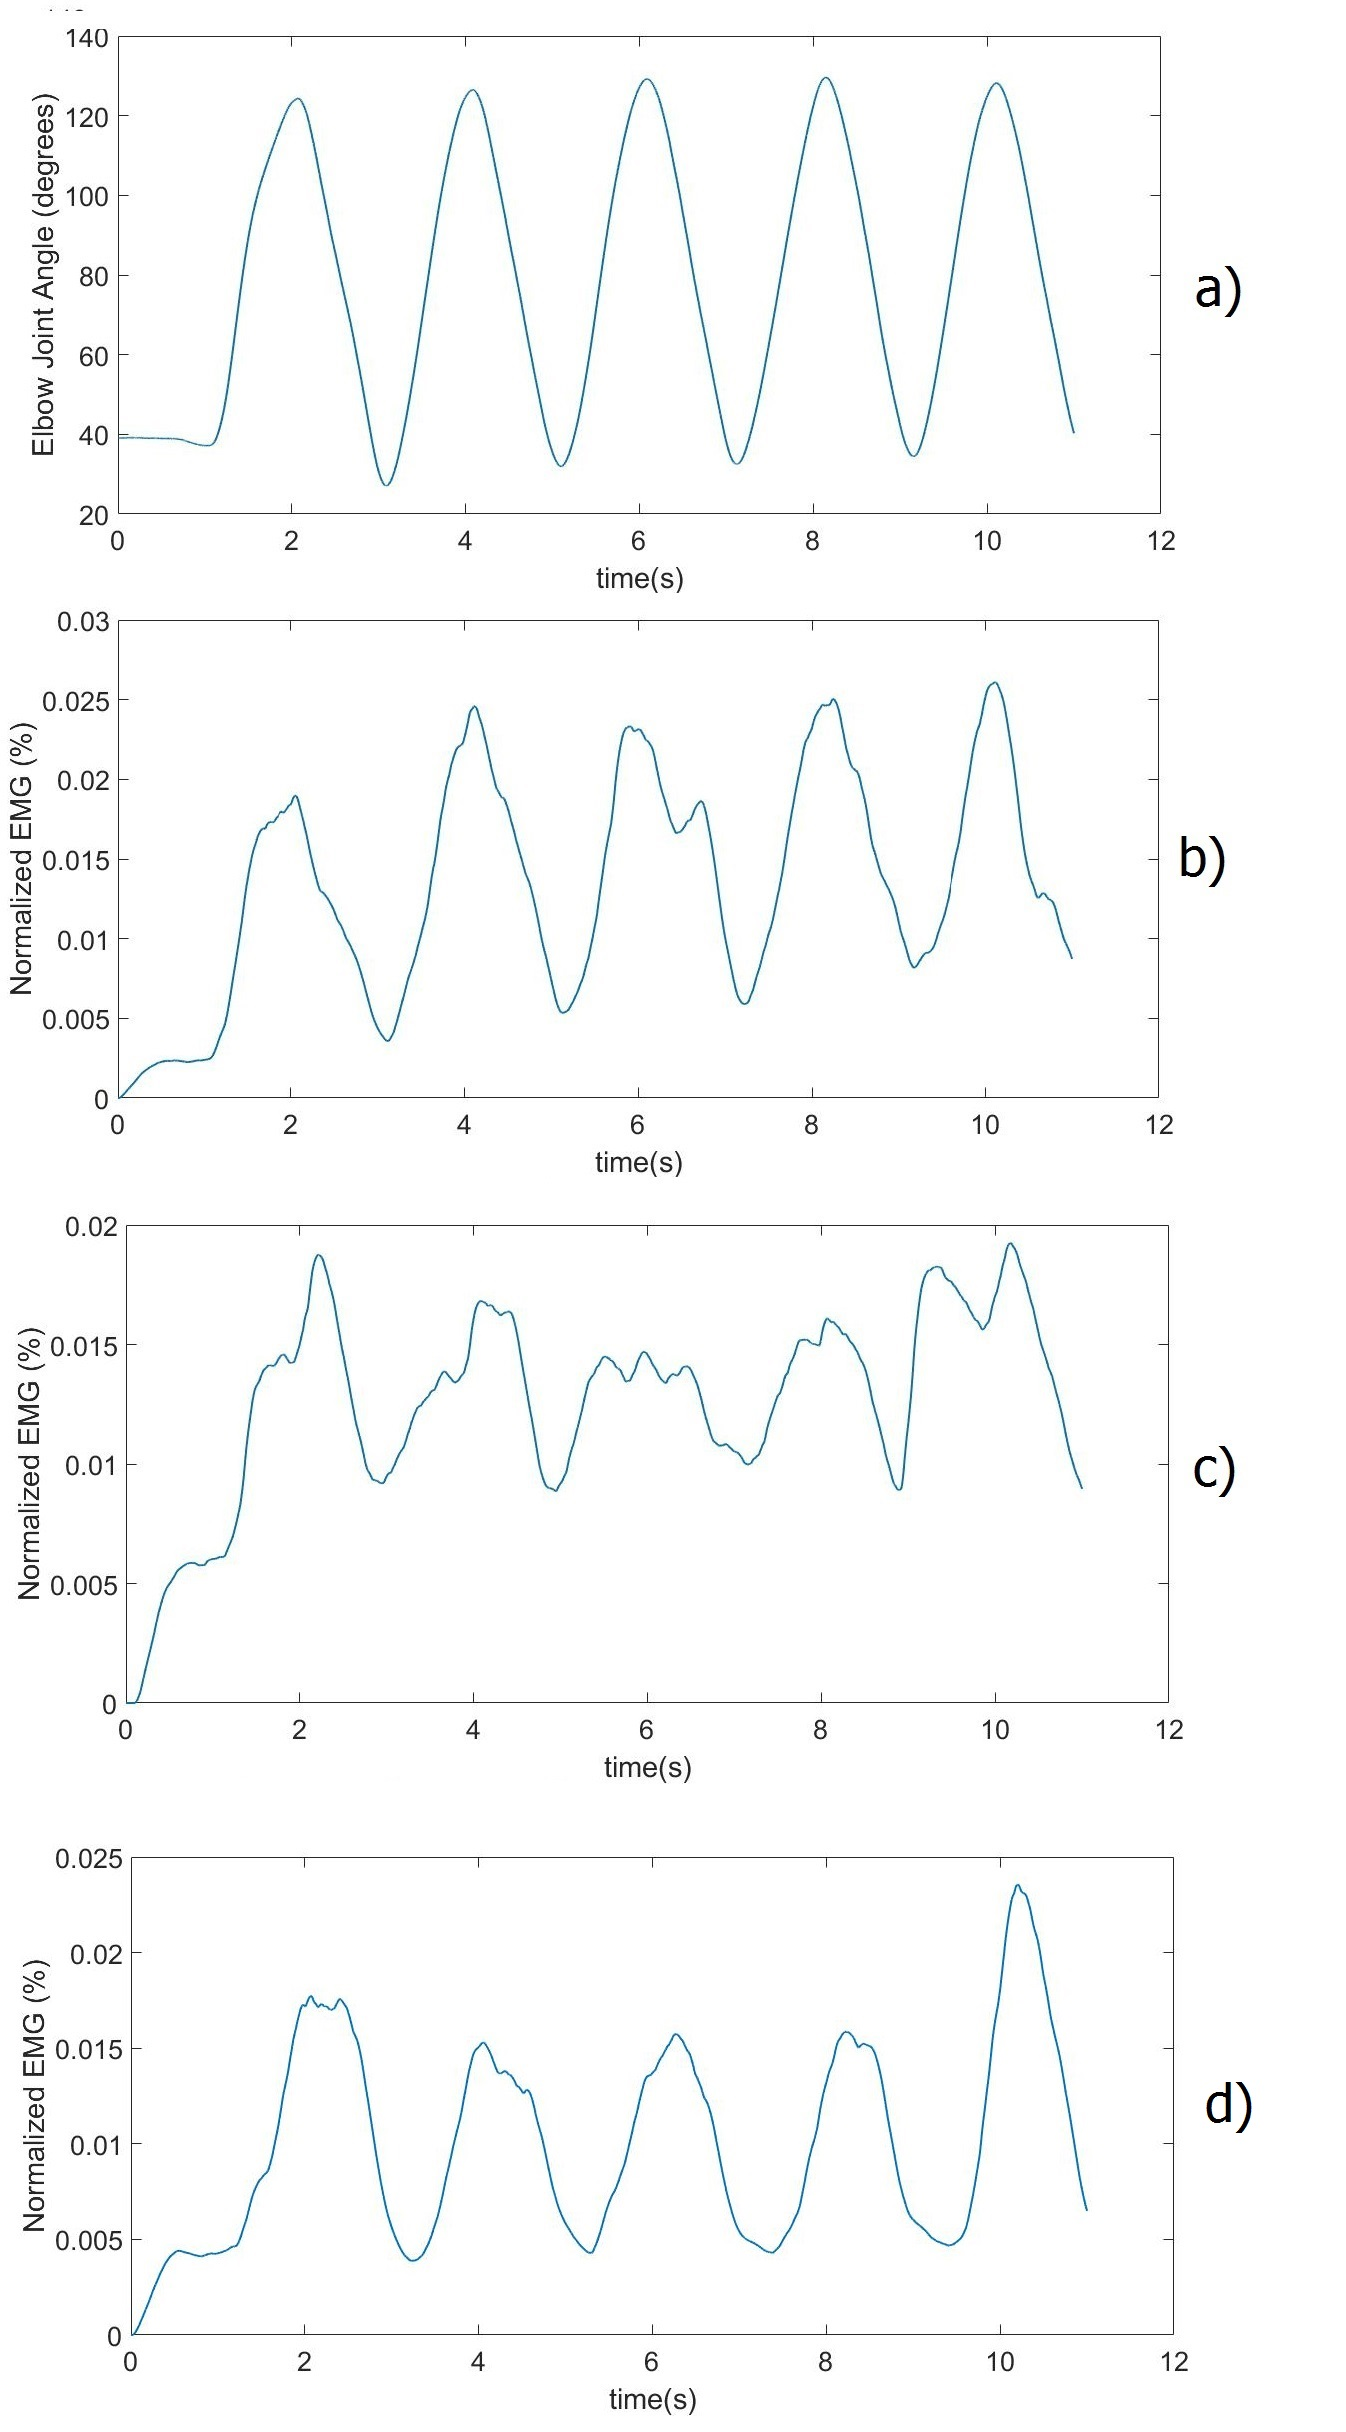
\includegraphics[height = 0.8\textheight]{Images/Angle_and_EMGs.jpg}
      \caption{a) Joint angle for the continuous movement with no extra weight, recorded with the IMU; sEMG values for the b) biceps brachii, c) triceps brachii and d) brachioradialis for the continuous movement with no extra weight.}
      \label{Angle and EMG}
   \end{figure}


\section{Linear System Modeling}

\begin{figure}[thpb]
      \centering
      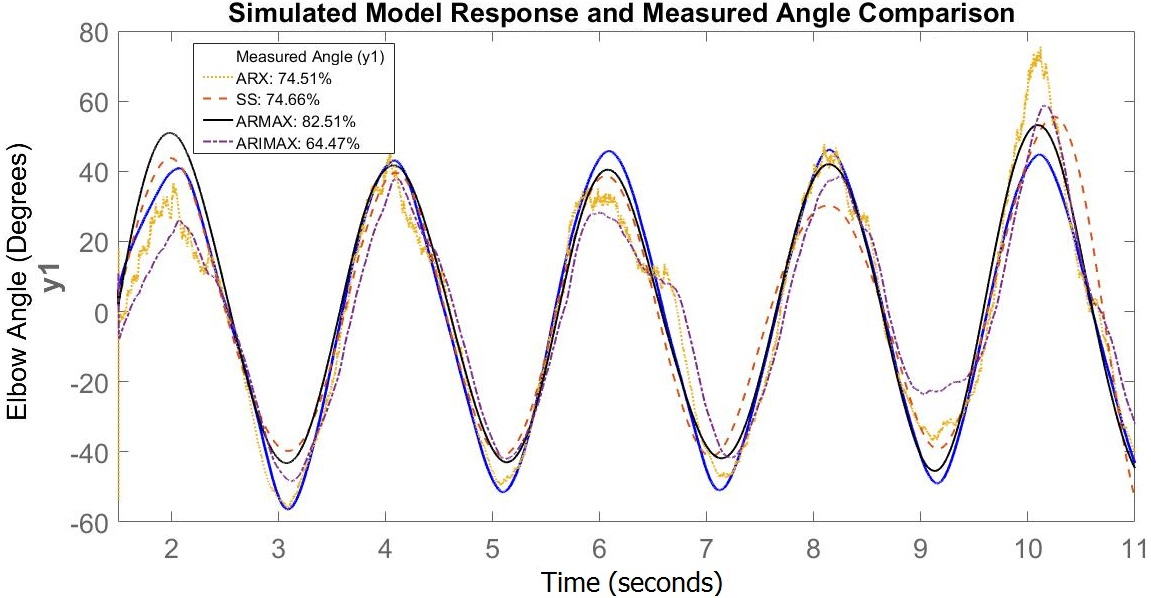
\includegraphics[scale=0.5]{Images/Models_comparison_5.jpg}
      \caption{Estimated elbow angle using the models responses compared to the elbow angle measured with the IMU. The estimated models were ARX, State Space, ARMAX and ARIMAX.}
      \label{Models Comparison}
   \end{figure}

It was assumed that the arm has the same model with different inertia parameters for the different weights attached to the arm of the subject arm. Considering a simple model of the elbow (arm with only 1 degree of freedom): 

\begin{equation}\label{eq:simpleModel}
T = (J + M\cdot L^2)\cdot \ddot{\theta}  + B \cdot \dot{\theta}  + (m\cdot l + M \cdot L) \cdot g \cdot cos(\theta)
\end{equation}


Where T is the elbow joint torque, J is the forearm inertia, B is the damping factor of the joint, m is the forearm mass, M is the dumbbell's mass, g is the gravity force and \(\theta\) is the joint angle. From this simple model it is easy to infer that, by changing the dumbbell's mass, the arm model parameters also change.

Four different modeling techniques were applied to determine which one best estimated the model that provides the elbow angle as an output taking the three EMG signals as inputs. These modeling techniques were: Auto-Regressive with Exogenous Input (ARX), Auto-Regressive Moving-Average with Exogenous Input (ARMAX), Auto-Regressive Integrated Moving-Average with Exogenous Input (ARIMAX) and State Space (SS).

To determine the best modeling technique, 10 models of each type were created with random parameter orders. Their estimation of the elbow joint angle was compared with each other. The model with the best fit value was chosen.  

With the model estimation technique chosen, it is necessary to determine the order of its parameters. To determine the chosen model order, 400 random combinations were tested for each data set with order values going from 0 to 10. The order chosen was the one that gave the best fit (see eq. \ref{eq:NRMSE}) between the estimated value and the one measured by the experiment. The coefficients of the models were estimated using time-domain data in Matlab\textsuperscript{\textregistered} (The Mathworks Inc, USA), minimizing a quadratic prediction error criterion.

To determine the best fit the normalized Root-mean-square error (NRMSE)  was used:
\begin{equation}
\label{eq:NRMSE}
NRMSE = 100*\left(1- \frac{||y-\hat{y}||}{||y-mean(y)||}\right)
\end{equation}

Where $y$ is the reference signal and $\hat{y}$ is the signal being evaluated.

\subsection{Results}

Figure \ref{Models Comparison} compares the different models with measured elbow angle and shows the fitness value for each data set.
The ARMAX model has the highest fitness value. For this reason it was the chosen model for the consequent estimations.

The ARMAX model has the following form:

\begin{equation}
A(q)y(t) = B(q)u(t-n_k)+C(q)e(t)
\end{equation}


Where y(t) is the output at time t, angle of the elbow joint, in this case; u(t) are the inputs, being the processed sEMG values from biceps brachii, brachioradialis and triceps brachii; e(t) is the white-noise disturbance; \(n_k\)  is the delay for each input; q is the delay operator; A, B and C are the model coefficients, defined by:

\begin{equation}
A(q) = 1 + a_1q^{-1}+\dots+a_{n_a}q^{-n_a}
\end{equation}
\begin{equation}
B(q) = 1 + b_1q^{-1}+\dots+b_{n_b}q^{-n_b+1}
\end{equation}
\begin{equation}
C(q) = 1 + c_1q^{-1}+\dots+c_{n_c}q^{-n_c}
\end{equation}


Where \(n_a\) is the system's number of poles; \(n_b\) is the number of zeroes plus one; \(n_c\) is the number of C coefficients.

The coefficient orders were calculated and can be found in table \ref{ta:order}.

\begin{table}[h]
\caption{Model parameters orders for each subject.}
\label{table_example}
\begin{center}
\begin{tabular}{|c|c|c|c|c|}
\hline
 & \(n_a\) & \(n_b\) & \(n_c\) & \(n_k\)\\
\hline \hline
Subject 1 & 1 & 1, 1, 4 & 1 & 8, 7, 0\\
\hline
Subject 2 & 1 & 1, 1, 4 & 1 & 8, 7, 0\\
\hline
Subject 3 & 1 & 1, 1, 4 & 1 & 8, 7, 0\\
\hline
Subject 4 & 1 & 1, 1, 4 & 1 & 8, 7, 0\\
\hline
Subject 5 & 1 & 1, 1, 4 & 1 & 8, 7, 0\\
\hline
Subject 6 & 1 & 1, 1, 4 &1 & 8, 7, 0\\
\hline
Subject 7 & 5 & 10, 3, 2 & 6 & 5, 3, 4\\
\hline
\end{tabular}
\end{center}

\label{ta:order}
\end{table}

\begin{figure}[thpb]
      \centering
      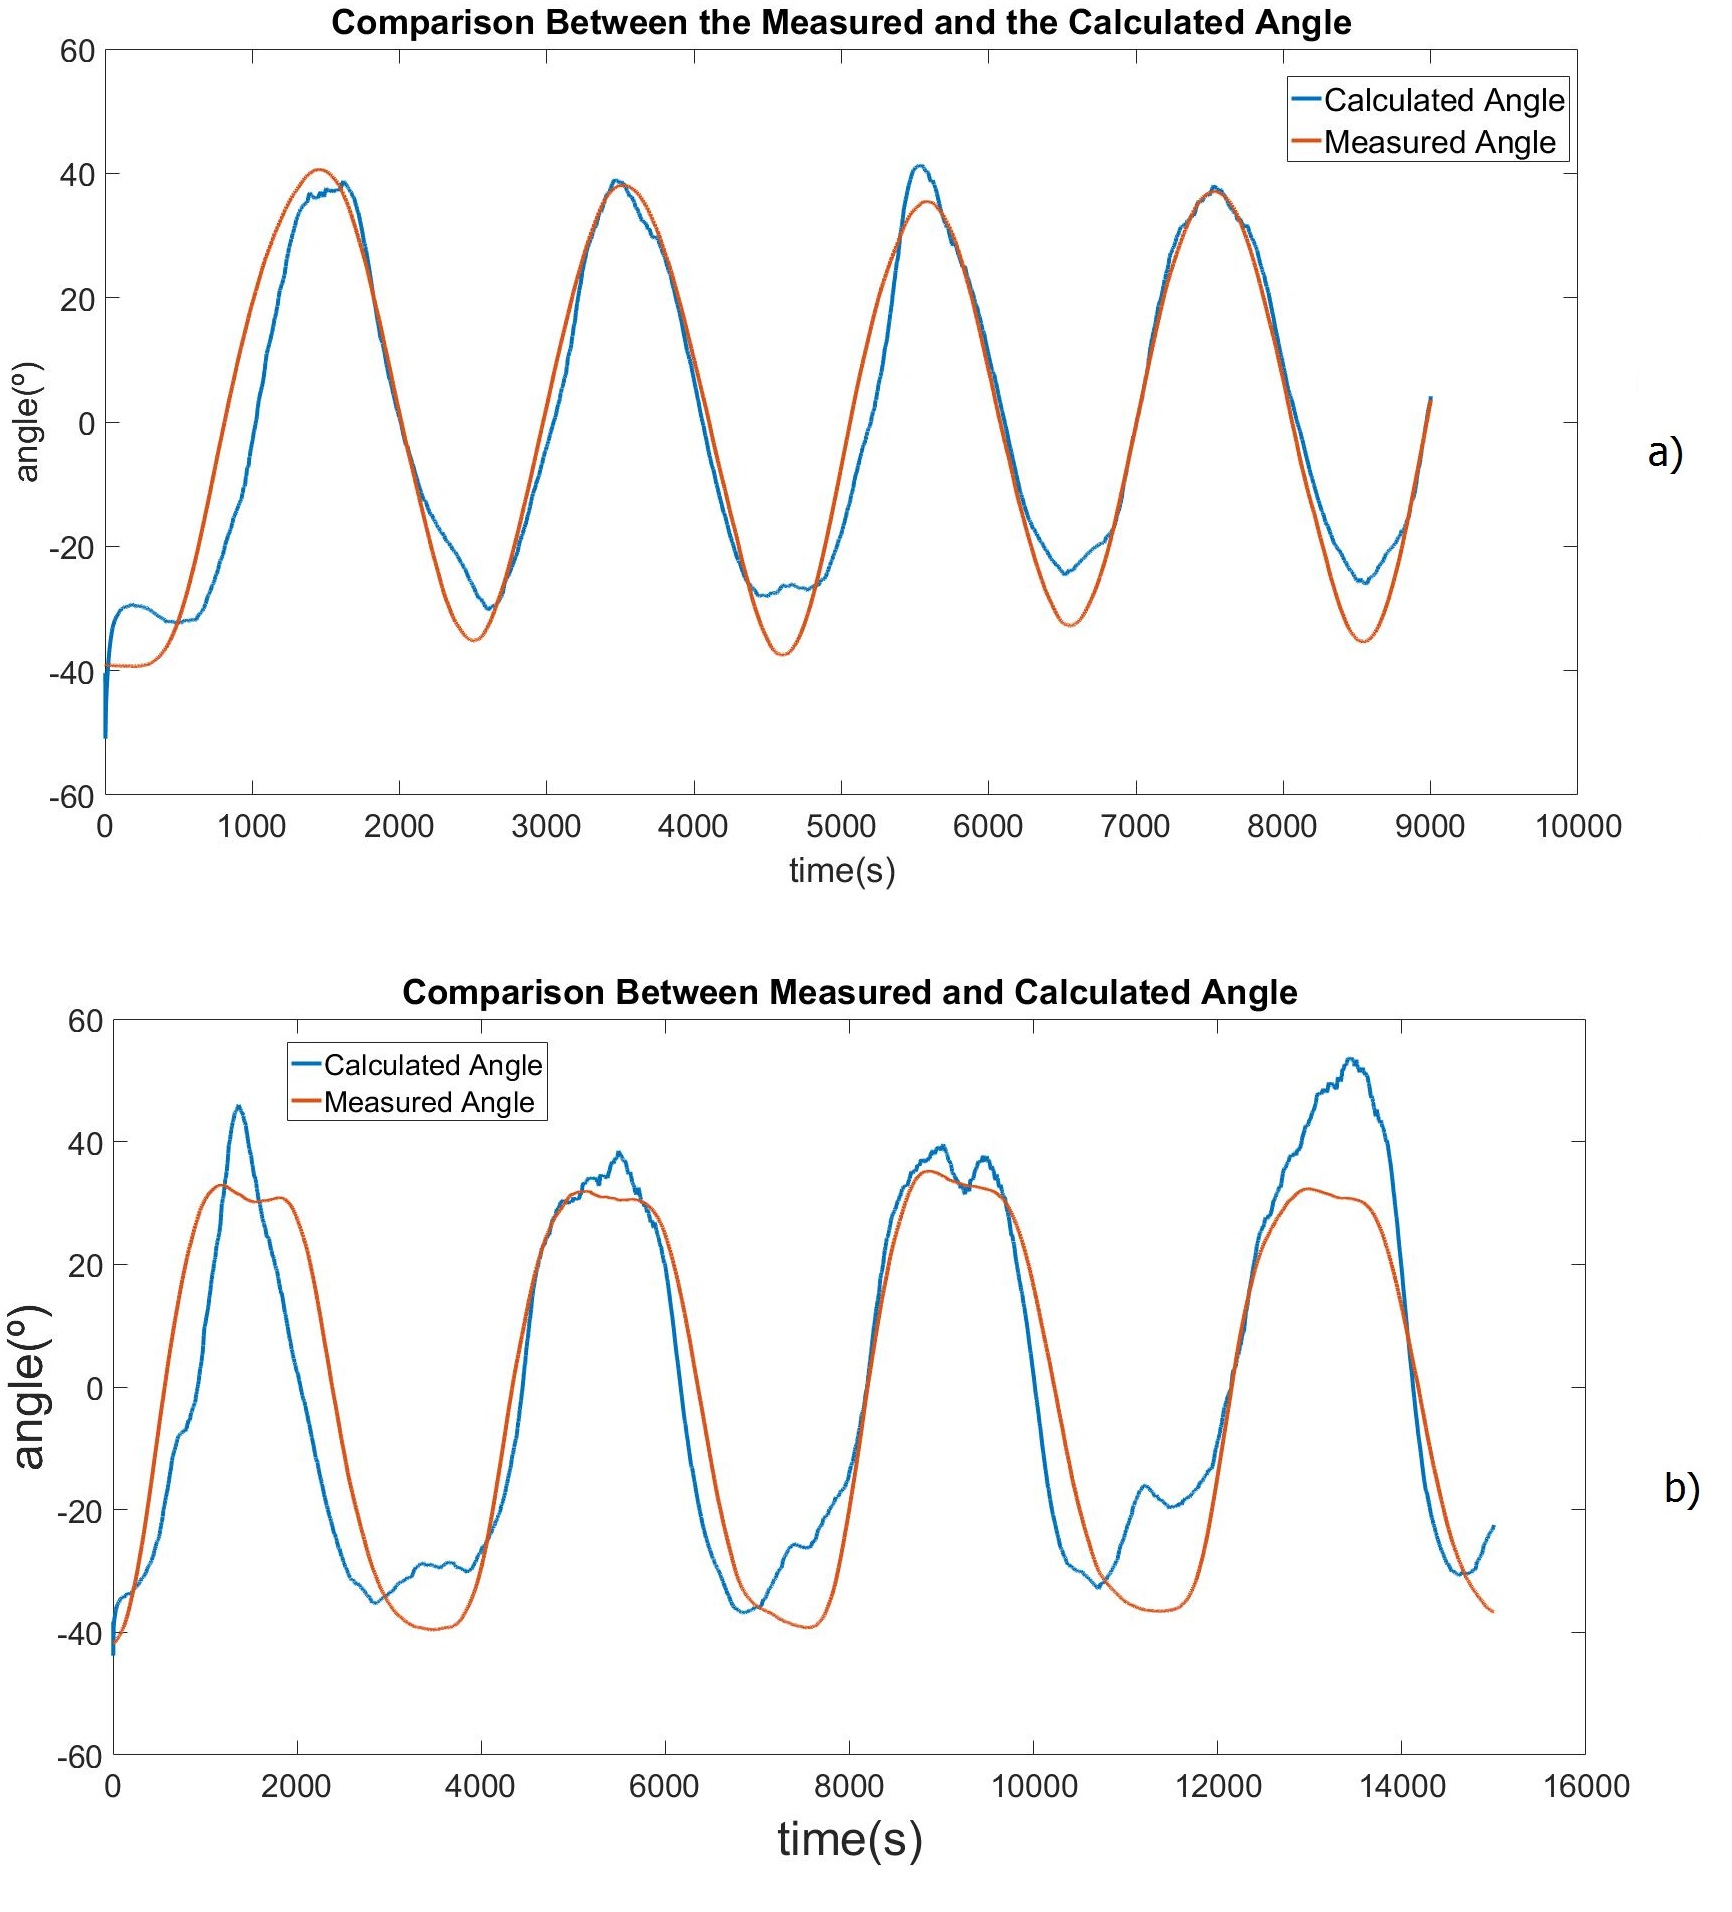
\includegraphics[scale=0.3]{Images/3kg.jpg}
      \caption{Comparison between the measured angle of the elbow joint and the angle calculated through the use of the estimated model, for subject 5. a) shows the comparison for the continuous movement and b) the comparison for the discrete movement}
      \label{Angle Comparison}
   \end{figure}

Using the values from table \ref{ta:order} as the ARMAX model orders, it was possible to calculate the model for elbow joint angle using the three sEMG measurements and compare it to the experimentally measured values. As an example, figure \ref{Angle Comparison} shows a comparison between the calculated and measured angle, for continuous and intermittent movement, for subject 5.

With the ARMAX model calculated for the test subjects, we aimed at validating the model. Using the same model order and parameters previously calculated we estimated the response of the system using a second batch of recorded data. An example of the result of this process can be seen in figure \ref{Validation Procedure}, where the model calculated for the subject number 3 was used to estimate the elbow joint angle using the input data acquired from the second day of testing.

\begin{figure}[thpb]
      \centering
      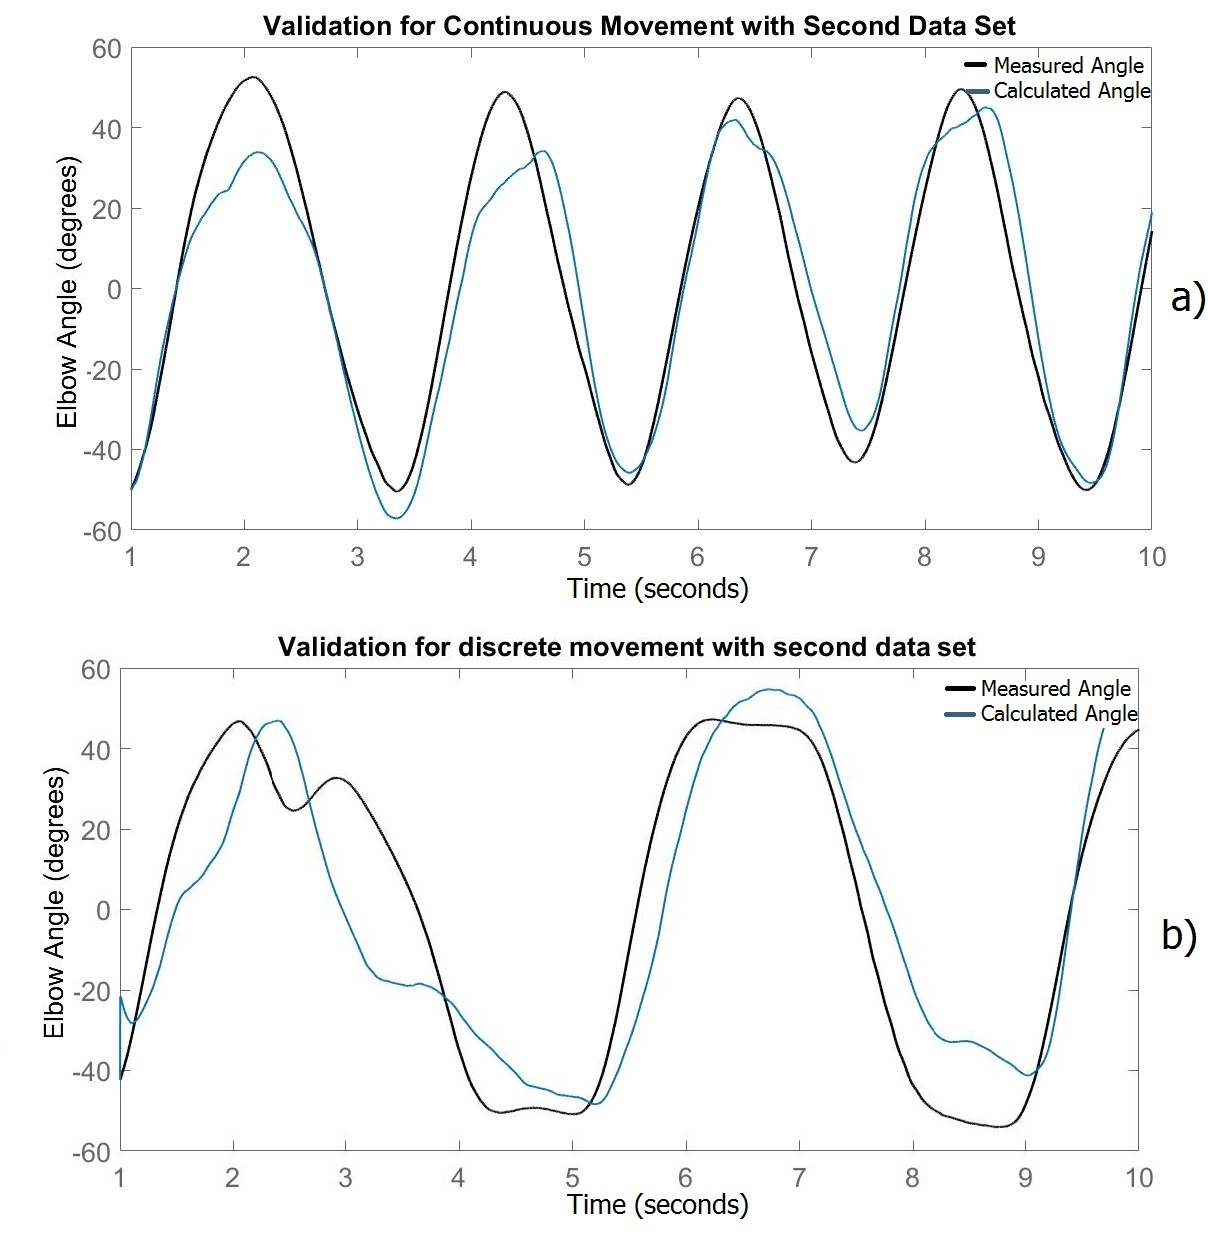
\includegraphics[scale=0.5]{Images/validation.jpg}
      \caption{Validation procedure to determine if the calculated model can be applied to the same test subject for tests made in different days. a) shows the comparison for the continuous movement and b) the comparison for the discrete movement}
      \label{Validation Procedure}
   \end{figure}

To better determine the accuracy of the model, two performance parameters were used: The correlation and the root-mean-square error (RMSE)  between the estimated and the measured elbow joint angles. Table \ref{ta:corr} shows the accuracy evaluation parameters for every test subject and every test set.


\begin{table}[h]
\caption{Correlation factor and Root-mean-square error for the estimated and measured angle values}
\label{table_example}
\begin{center}
\resizebox{\columnwidth}{!}{%
\begin{tabular}{|c c|c c|c c|c c|c c|}
\hline
\multicolumn{2}{|c|}{} & \multicolumn{4}{c|}{Calibration Test} & \multicolumn{4}{c|}{Validation Test} \\
\hline
\multicolumn{2}{|c|}{} & \multicolumn{2}{c|}{Continuous} & \multicolumn{2}{c|}{Intermittent} & \multicolumn{2}{c|}{Continuous} & \multicolumn{2}{c|}{Intermittent} \\
\hline
\multicolumn{2}{|c|}{} & Correlation & RMSE & Correlation & RMSE & Correlation & RMSE & Correlation & RMSE\\
\hline \hline

& 0 kg &0.8914 &15.61 &0.8218 &20.65 & 0.8966 & 29.85 & 0.9107 & 18.44 \\
Subject 1 & 1.5 kg &0.7761 &16.66 &0.8251 & 15.19 &0.825 &18.48 & 0.47 & 34.9\\
& 3 kg &0.9497 &13.82 &0.9011 &16.85 & 0.6123 & 29.13 & 0.8488 & 18.85\\
\hline

& 0 kg &0.9285 &11.29 &0.9659 &9.51 & 0.8249 & 19.28 & 0.941 & 20.43\\
Subject 2 & 1.5 kg &0.8011 &26.33 &0.897 & 16.59 & 0.8735 & 17.48 & 0.8935 & 22\\
& 3 kg &0.9314 &11.85 &0.9368 &13.7& 0.8666 & 16.32 & 0.8906 & 18.61\\
\hline

& 0 kg &0.8682 &19.47 &0.9123 &16.29 & 0.9033 & 18.04 & 0.8572 & 20.17\\
Subject 3 & 1.5 kg &0.9383 &16.61 & 0.9413& 12.42 & 0.922 & 16.045 & 0.9109 & 16.61\\
& 3 kg &0.9341 &13.66 &0.9602 &10.43& 0.9852 & 16.4 & 0.9048 & 17.16\\
\hline

& 0 kg &0.8806 &19.63 &0.88 &21.56 & 0.752 & 29.62 & 0.8931 & 21.87\\
Subject 4 & 1.5 kg &0.9408 &16.052 &0.9199 &17.95 & 0.3377 & 66.23 & 0.7704 & 39.44\\
& 3 kg &0.9608 &17.628 &0.862 &21.86 & 0.6104 & 139.73 & 0.7643 & 53.31\\
\hline

& 0 kg &0.8974 &18.805 &0.873 &24.68 & 0.9407 & 44.398 & 0.9192 & 16.322\\
Subject 5 & 1.5 kg &0.9233 &27.954 &0.823 &17.31 & 0.8801 & 15.427 & 0.8784 & 16.912\\
& 3 kg & 0.9621&7.286 &0.9239 &10.89& 0.8652 & 21.81 & 0.8445 & 24.316\\
\hline

& 0 kg &0.9256 &14.311 &0.9029 &20.76 & 0.8793 & 34.11 & 0.9258 & 53.08\\
Subject 6 & 1.5 kg &0.8184 &19.37 &0.828 &19.93 & 0.7782 & 21.96 & 0.9317 & 26.05\\
& 3 kg & 0.8323 & 19.13 &0.9169 &16.3 & 0.7722 & 102.16 & 0.8043 & 31.88\\
\hline

& 0 kg &0.9147 &18.515 &0.9057 &15.48 & 0.8063 & 19.335 & 0.9 & 15.815\\
Subject 7 & 1.5 kg &0.9066 & 12.424&0.9411 & 11.85 &0.8728 & 17.035 & 0.887 & 18.509\\
& 3 kg &0.9194 &12.857 &0.949 &12.6 & 0.7825 & 18.16 & 0.931 & 15.12\\
\hline

\end{tabular}%
}
\end{center}

\label{ta:corr}
\end{table}

\subsection{Non-Linear System Modeling}

\subsection{Results}

\subsection{Discussion and Conclusions}

This chapter proposed a method for determining the elbow joint angle based on the measurement of the sEMG of biceps brachii, triceps brachii and brachioradialis from 7 test subjects. The arm model was estimated using the data collected from the experiment and a system identification method, more specifically, ARMAX. Using the acquired sEMG data as input to the estimated model, it was possible to obtain an estimation of the elbow angle. Using the data from the IMU (real angle value) it was possible to validate the estimation based on sEMG.

The experimental data showed that it is possible to use only the EMG data to estimate a correlation between joint angle and sEMG values. Even though estimating one model for continuous movement and another one for discrete movement gives higher precision, it is possible to calculate a single model for both movements.

As stated before, by lifting different weights the model parameters are altered.
For the same test subject the A(q) and C(q) parameters (see eq. 3) maintained values with less than 1\% difference from one another, while the B(q) values assumed a greater range of values.

Even for different subjects, the estimated A(q) and C(q) parameters also had a difference of less than 1\% from one another.

From the seven subjects, six of them could be estimated by an ARMAX model with the same parameters order. The test subject with different order parameters was the one that presented the worst readings of the brachioradialis muscle EMG. Because of that, a lot of noise is introduced, requiring a higher order system to overcome the modeling errors. The brachioradialis is the most difficult muscle to read the sEMG signals compared to the biceps brachii and the triceps brachii. This difficulty is due to the muscle short length causing the electrodes to stay close to the tendon, which induces  reading errors. Not coincidentally, this test subject was the one with smaller stature.

The repeatability of the model was successful for the cases studied in this work, even though it is possible to note that the model is not as precise as it was for the calibration procedure.

In future works it will be studied if it is possible to define one single estimated model for each subject, independent of the weight being lifted, or even one global model that is capable of estimating joint angles for a big range of individuals. The calculated models will be used for the control of an EMG-driven upper limb exoskeleton.

\chapter{Proportional EMG-Driven Angle Control}
\label{ch:ProportionalControl}

Many authors applied successfully a proportional EMG control for a mechanism (e.g. \cite{Bottomley411}). Hogan \cite{1103644} stated that, for contractions of the muscle below 30\% of the maximum voluntary contraction, the relative force applied by the biceps muscle to the elbow joint and the EMG signal can be considered as proportional. 

Lets assume a simplified model of the arm with one degree of freedom on the elbow joint. 

\begin{equation}\label{eq:simpleModel}
T = (J + M\cdot L^2)\cdot \ddot{\theta}  + B \cdot \dot{\theta}  + (m\cdot l + M \cdot L) \cdot g \cdot cos(\theta)
\end{equation}


If we assume low speed and low acceleration, the equation can be simplified to:

\begin{equation}\label{eq:kcos}
T = K \cdot cos(\theta)
\end{equation}

\begin{equation}
K = (m\cdot l + M\cdot L)\cdot g
\end{equation}

Where K is the coefficient for the gravity-related forces.

This equation states a direct relationship between joint angle and torque and consequently, for low muscle activation levels, joint angle and EMG magnitude.

From the experiments developed at chapter \ref{ch:preliminarExperiment}, a powerful relation between the elbow angle and the sEMG signal can be observed, especially at the test set where the user is carrying no extra weight in his hand, shown in figure \ref{EmgAngleDirect}.

\begin{figure}[thpb]
      \centering
      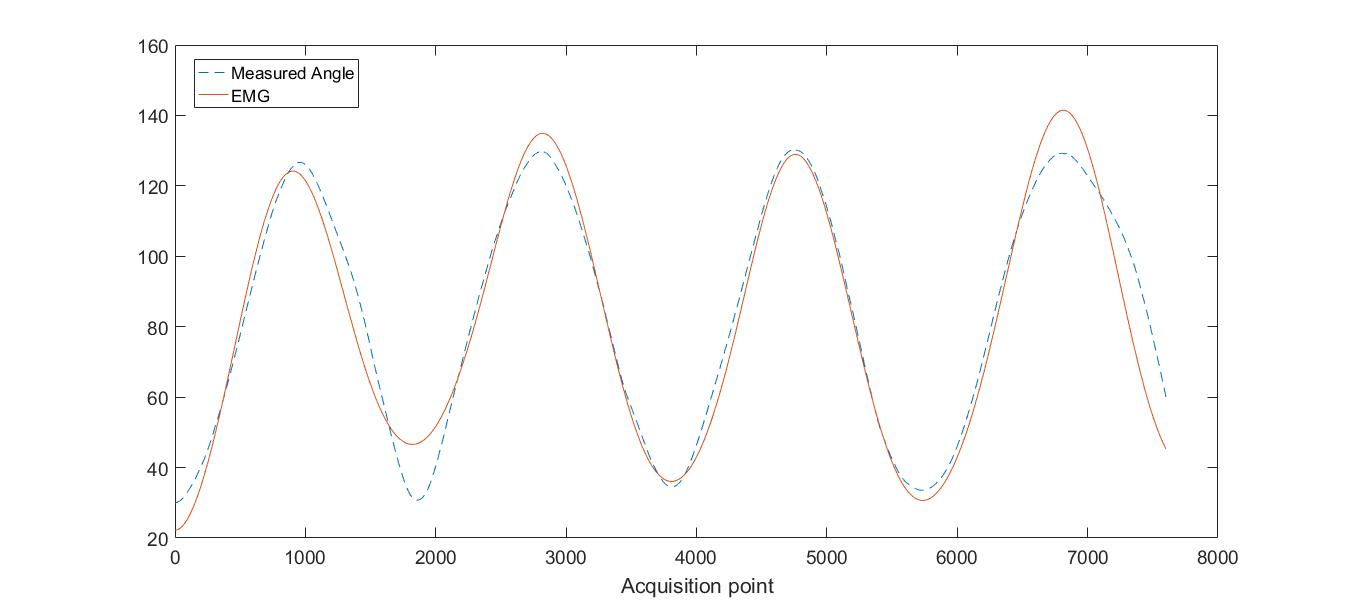
\includegraphics[scale=0.35]{Images/EmgAngleDirect.jpg}
      \caption{Comparison between the measured elbow angle and the EMG values for the continuous movement. The EMG values were multiplied by a constant for better visualization.}
      \label{EmgAngleDirect}
   \end{figure}
   
   The correlation between these two signals is 97.78\%. It shows that, at least for the configuration of the proposed experiment, there is a high correlation between the EMG signal and the elbow joint angle.
   
   The first problem of this relation appears when comparing the EMG signals with the intermittent movement. See figure \ref{EmgAngleInt}.

\begin{figure}[thpb]
      \centering
      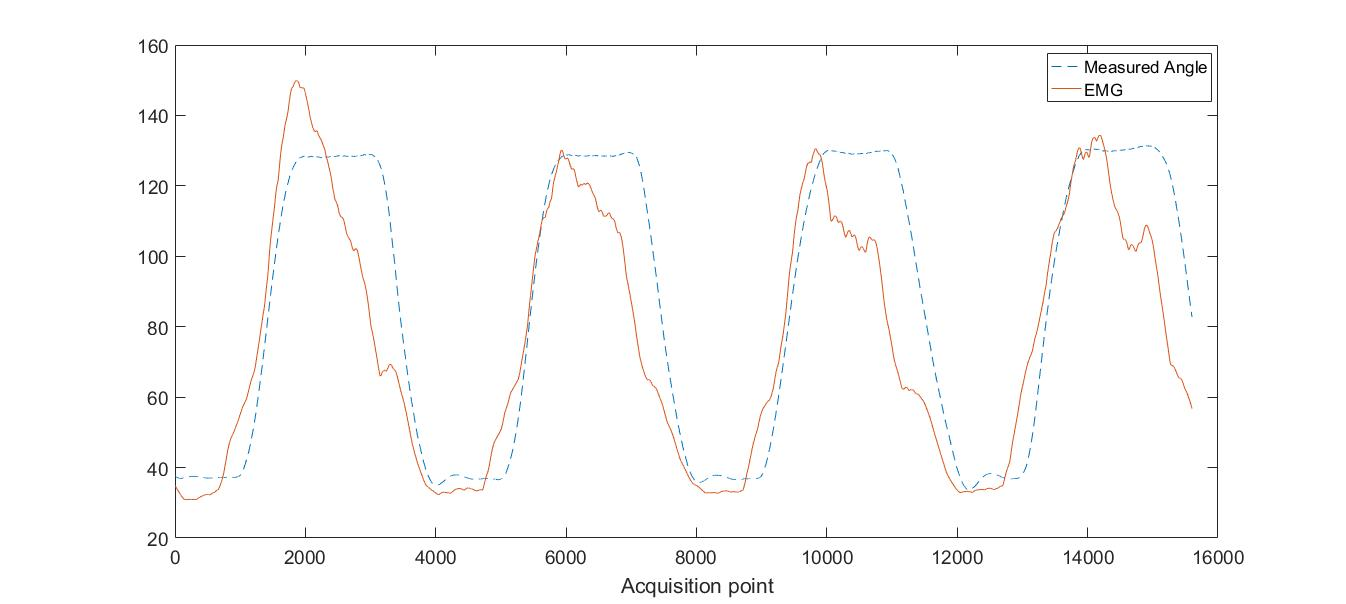
\includegraphics[scale=0.35]{Images/EmgAngleInt.jpg}
      \caption{Comparison between the measured elbow angle and the EMG values for the intermittent movement. The EMG values were multiplied by a constant for better visualization.}
      \label{EmgAngleInt}
   \end{figure}
   
   As the image shows, for the upward movement, there is a proportional relation between the EMG values and the angle of the elbow joint. When the elbow joint stays in a static angle, the EMG magnitude lowers, even without elbow movement. 
   
   
   To address this problem, further investigations must be made. Two main ideias will be explored. The first one is to use the Time Domain analysis of the EMG signal. The TD analysis is commonly used in pattern recognition for EMG signals. It uses the Mean Absolute Value,
Zero Crossing, Slope Sign Changes and Waveform Length of the signal to acquire more information about the user's intention of movement. Another ideia is to use the wavelet analysis to the EMG signal. The wavelet analysis is extensively used in EMG pattern recognition systems. It analyses a larger bandwidth than just the 1Hz to 3Hz commonly used in EMG proportional control. By analyzing higher frequencies, it is possible to acquire more information about the intention of movement. "Borrowing" this technique to the proportional control, we may be able to detect the intention to make an extension movement and then using the proportional control to determine the desired position of the joint.

\chapter{Hybrid Control}
\label{ch:Hybrid Control}

The hybrid control is a control method that comprises more than one sensor type. The one that will be applied to this work will use force sensors attached to the arm of the exoskeleton. 

The values measured by the sensors will define a dynamic area. We define dynamic area as a set of a number of activities to be performed based on a set of combinations from the readings of the sensors. It is based on the dynamic area proposed by Philipson \cite{Philipson1985} shown in figure \ref{Movement space}
The control will be based in a dynamic area composed of three levels for each of the sensors: The sEMG sensor and the force sensor (figure \ref{DynamicAreaHybrid}). The convention for the force sensor signal is positive for when the user is applying a force to the exoskeleton in the direction of the flexion movement and negative in the direction of extension movement. The sEMG sensor is placed at the muscle responsible for the flexion movement.

\begin{figure}[thpb]
      \centering
      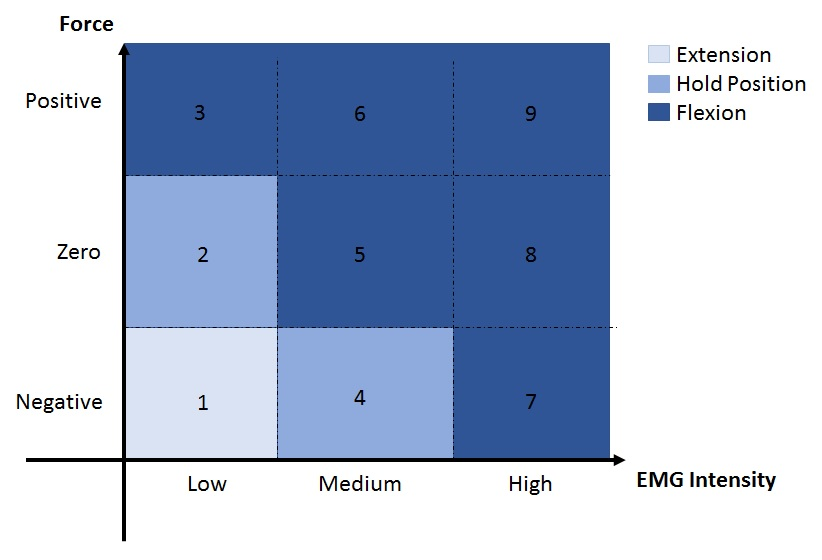
\includegraphics[scale=0.6]{Images/DynamicAreaHybrid.jpg}
      \caption{Dynamic area for the hybrid control.}
      \label{DynamicAreaHybrid}
   \end{figure}

The dynamic area shows the desired motion for the mechanism according to the level of the inputs from both sensors.

Each area, denoted by a number in the figure, represents a different situation for the user. The reasoning behind the decision making of the controller is as follows:

\begin{itemize}
\item 1: No movement intention but there is a load forcing the limb to an extension movement.
\item 2: There is no movement intention nor load forcing the limb to extension or flexion movement.
\item 3: The user is flexing his limb and supporting the entirety of the load as well as forcing the exoskeleton to a flexion movement.
\item 4: User has the intention to maintain his limb position and its arm is being supported by the exoskeleton.
\item 5: The user's strength is in equilibrium with the weight of the load, but the exoskeleton must act to support the user's arm, avoiding fatigue.
\item 6: Same as 3
\item 7: Intention of movement, but the user is unable to lift the load using his own strength.
\item 8: Intention of movement, but the user's strength is in equilibrium with the weight of the load.
\item 9: The user is carrying the weight by himself and forcing the exoskeleton in the flexion direction.
\end{itemize}

This way it is possible to implement a set of rules for the controller:

If the signal from the sEMG is low, there is no intention of movement from the user. This way, the user's limb offers no resistance to external loads. If any external load is applied the user's limb will move in the same direction as the force applied and the exoskeleton should move in that same direction, offering no resistance.

If the signal from the sEMG is in an intermediate level, it characterizes the user's intention to maintain its limb position. If the force sensor measures a negative force, the exoskeleton is supporting the user's limb. Therefore, it must maintain its position. If the force sensor measures no force, the user is carrying the load using his own strength, potentially causing muscular fatigue. The exoskeleton must act in the extension direction until it supports the user's limb, maintaining a comfortable position for the user. When the force sensor measures a positive force, the user's limb is supporting the entirety of the load and forcing the exoskeleton into a flexion movement. The exoskeleton perform a flexion movement to alleviate the load applied to the user's limb.

If the signal from the sEMG is high, it characterizes a movement intention from the user. If the force sensor measures a negative force, the user's strength is inferior to the load, so the exoskeleton must assist the user's movement. If the force sensor measures no force, the user's strength is sufficient to maintain the limb in a static position, but it will soon cause fatigue. The exoskeleton must act to support the user's limb and the load. If the force sensor measures a positive force, the user is carrying the load and forcing the exoskeleton in to a flexion movement. The exoskeleton must act to alleviate the load in the user's limb.

\include{Paper}

\chapter{Courses and Schedule}

\section{Courses}

\subsection{PME5018 - Projeto Integrado de Sistemas Mecânicos}

This course offers a great understanding of the project of a mechanical system. Not focusing only in the calculations and design of the product, this course presents a systemic and conceptual analysis of the project spiral. This course was of great importance for the design of ETMICAE since this project can later become a marketable product.

Grade: A

\subsection{PTC5721 - Controle Ótimo I}

This course presents the basic concepts for the Optimal Control Theory using Dynamic Programming and Variational calculus. Even with limited application in my current project objectives, this course offered greater understanding of the control theory. Heavily focused on a mathematical approach to the solution of the control problems. The tools and knowledge acquired through this course can be used in later implementations and developments of the exoskeleton control presented in this work.

Grade: C

\subsection{PMR5014 - Controle Não Linear Aplicado a Sistemas \\ Mecânicos e Mecatrônicos}

This course presents control techniques designed for non-linear systems, where the applications of classic control methods are not satisfactory. Differing from the Optimal Control course, this one offers a more practical and computational approach to the control problem. During the course, many control exercises were proposed to the students and solved through the use of MATLAB\textsuperscript{\textregistered}.  The exoskeleton presents some non-linearities such as viscous friction and gravitational forces. For this reason, the design of a non-linear controller can be favorable for a good control of the exoskeleton. 
%During the course, the design and analysis of a non-linear control method for an upper limb exoskeleton with a  one degree of freedom was made.

Grade: B

\subsection{PMR5004 - Fundamentos do Projeto de Sistemas \\ Mecânicos}

Focused on the basic and executive project steps of a mechanical system. Differing from the other mechanical project course, this one heavily focuses on mathematical tools for the selection and design of mechanical parts and machines. This course was of great importance for the design of ETMICAE and future developments on the mechanical structure of the exoskeleton since it offered a deeper understanding and mastery of mechanical design.

Grade: B

\subsection{PMR5005 - Biomecatrônica e Biorobótica}

This course offers a great overview of Biomechatronics and Biorobotics, presenting concepts and theories of the human motor control and human dynamics and how to develop robotic systems for assistance and rehabilitation. The information obtained through this course was of great importance to better understand the major breakthroughs and challenges to the exoskeleton and assistive technologies, better directioning this present work. At the end of this course, the first iteration of a system identification method for the upper limb was applied, which would later develop into the elbow angle estimation chapter present in this work.

Grade: A

\subsection{PMR5240 - Sensores, Atuadores e Problemas Inversos Bayesianos em Medicina}

This course offers an in-depth approach to technologies and sensors applied to medicine problems, such as ultrasound, image analysis and electrical impedance tomography. Even though the subject strays from the main focus of this work, it presented many different technologies and strategies that can be later applied to the control of an exoskeleton (e.g. using ultrasound to determine the muscle contraction and, consequently, a motion intention).

Grade: A

% Adicionado só para ter uma melhor formatação

\clearpage

\section{Schedule} 

\begin{figure}[thpb]
      \centering
      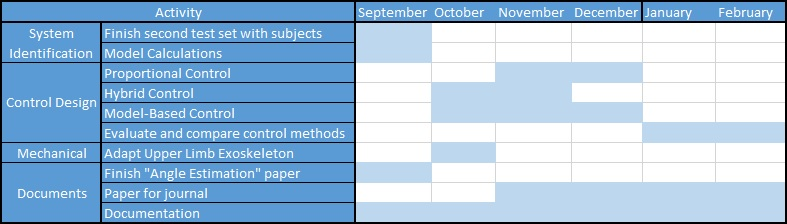
\includegraphics[width = \textwidth]{Images/Schedule.jpg}
      \caption{Schedule}
      \label{Schedule}
   \end{figure}


% ========== Referências ==========
% --- IEEE ---
%	http://www.ctan.org/tex-archive/macros/latex/contrib/IEEEtran
%\bibliographystyle{IEEEbib}
\bibliographystyle{ieeetr}

% --- ABNT (requer ABNTeX 2) ---
%	http://www.ctan.org/tex-archive/macros/latex/contrib/abntex2
%\bibliographystyle{abntex2-num}

\bibliography{Bibliography}


% ========== Apêndices (opcional) ==========
%\apendice
%\chapter{}
%\chapter{Beta}


% ========== Anexos (opcional) ==========
%\anexo
%\chapter{Alpha}
%\chapter{}



\end{document}
